\documentclass{article}
\usepackage{dsfont, amsmath, amsthm}
\usepackage{graphicx} % Required for inserting images
\usepackage[hidelinks]{hyperref}  %To remove the red outline
\usepackage{tikz}
\usetikzlibrary{arrows.meta}
\usetikzlibrary{decorations.pathmorphing}
\usepackage{algorithm}
\usepackage{algpseudocode}
\usepackage{pgf} % For arithmetic operations in TikZ
\usepackage{comment}


\tikzset{
    nodo/.style={
        shape=circle,
        draw=black,
        line width=1,
        minimum size=7mm
    },
    arista/.style={
        line width=1,
        -{Latex[length=3mm]}
    }
}


\usepackage[a4paper, total={6in, 8in}]{geometry}

% AI stuff
\newcommand{\domain}{\mathds{D}}
\newcommand{\entities}{\texttt{ent}}
\newcommand{\consistsWith}{\texttt{cw}}
\newcommand{\charFunML}{\charactheristicFunction}
\newcommand{\aCircuit}{\mathcal{C}}

% Computational complexity stuff
\newcommand{\NP}{\textsc{NP}}
\newcommand{\NPhard}{\textsc{NP-hard}}
\newcommand{\NPcomplete}{\textsc{NP-complete}}
\newcommand{\sharpPhard}{\textsc{\#P-hard}}

% Sets and probability stuff
\newcommand{\R}{\mathds{R}}
\newcommand{\perm}{perm}
\newcommand{\aDistribution}{\mathcal{D}}
\newcommand{\expectancy}{\mathds{E}}
% Important names and stuff
\newcommand{\SHAPscore}{\textsc{SHAP-score}}
\newcommand{\aBayesianDistribution}{\mathcal{B}}
\newcommand{\set}[1]{ \{ #1 \} }

% Game Theory
\newcommand{\charactheristicFunction}{\nu}
\newcommand{\players}{\mathcal{I}}
\newcommand{\Shap}{Shap}
\newcommand{\assym}{\Shap^{assym}}

% DAG and Assym Notation
\newcommand{\toOr}{\pi} %topologicalOrder
\newcommand{\rel}{R} %relation
\newcommand{\union}{union}
\newcommand{\equivalenceClass}{[\pi]_{\rel}} %equivalenceClass
\newcommand{\eqClassSize}{eqClassTopos}
\newcommand{\equivalenceClassRep}{\mathsf{Rep}(\equivalenceClass)}
\newcommand{\numEqCl}{\#EC} %equivalenceClass formula
\newcommand{\unrEqCl}{UnrEC} %unrelated equivalenceClass formula
\newcommand{\heuristicASVFormula}{\frac{1}{|\topo(G)|} \sum_{\equivalenceClass \in eqCl(G, x_i)} (\charactheristicFunction(\toOr_{<i} \cup \{x_i\}) - \charactheristicFunction(\toOr_{<i})) \cdot |\equivalenceClass|} %New Formula
\newcommand{\eqClassSizes}{eqClassSizes} %unrelated equivalenceClass sizes formula
\newcommand{\leftPossibleOrders}{\#LO} %Left possible orders

%% Drawing graphs

\newcommand{\drawUnrelatedTreeWithColor}[5]{
    \node[circle, draw=#5] (#1) at (#2, #3) {#4};
    \pgfmathsetmacro{\x}{#2-2}
    \pgfmathsetmacro{\y}{#3-0.3} 
    \draw[#5, wiggly] (#2, \y)
        -- ++(-1,-1.6) 
        -- ++(2,0) 
        -- cycle;
    \node[text=#5] at (\x, \y) {#4 subtree};
}

\newcommand{\drawUnrelatedTree}[4]{
    \drawUnrelatedTreeWithColor{#1}{#2}{#3}{#4}{red}
}

\newcommand{\drawUnrelatedTreeWithTag}[6]{
    \drawUnrelatedTreeWithColor{#1}{#2}{#3}{#4}{#5}

    % Texto de nodos disponibles (más abajo del contorno)
    \pgfmathsetmacro{\ysubtree}{#3 - 0.3}
    \pgfmathsetmacro{\ytext}{\ysubtree - 2.0}
    \node[text=#5] at (#2, \ytext) {#6};
}


% Comments and stuff
%\definecolor{darkred}{rgb}{0.55, 0.0, 0.0}
%\usepackage[dvipsnames,svgnames,x11names]{xcolor}
\usepackage[backgroundcolor=orange, textcolor=black, textsize=tiny]{todonotes}
\newcommand{\santi}[1]{\todo[inline,caption={},color=blue!30]{{\bf Santi:} #1}}
\newcommand{\echu}[1]{\todo[inline,caption={},color=orange!30]{{\bf Echu:} #1}}
\newcommand{\sergio}[1]{\todo[inline,caption={},color=green!30, size=\footnotesize]{{\bf Sergio:} #1}} 
\newcommand{\sidesergio}[1]{\todo[caption={},color=green!30, size=\footnotesize]{{\bf Sergio:} #1}}
\newcommand{\aMechanism}[0]{\mathcal{D}}
\newcommand{\anAlgorithm}[0]{\mathcal{A}}

% Graphs and networks
\newcommand{\topo}{topos}
\newcommand{\numTopo}{\#topos}
\newcommand{\aBayesianNetwork}{N}
\newcommand{\parents}{\textit{Parents}}
\newcommand{\dtrees}{\emph{dtrees}}
\newcommand{\dtree}{\emph{dtree}}
\newcommand{\childNetwork}{\emph{Child}}
\newcommand{\cancerNetwork}{\emph{Cancer}}
\newcommand{\variableNetwork}[1]{\texttt{#1}}
\newcommand{\intersectionNode}{i_{\cap}}
\newcommand{\subtree}{s}


% Theorems %Traducidos 18/3
\newtheorem{example}{Ejemplo}
\newtheorem{theorem}{Teorema}
\theoremstyle{plain} %Nota amsthm es necesario para Theoremstyle
% \newtheorem{proposition}[theorem]{Proposition} Si lo hago de este modo todos compartirían el mismo contador y no quiero que eso pase. 
\newtheorem{proposition}{Proposición} 
\newtheorem{lemma}{Lema}
\newtheorem{corollary}{Corolario}
\newtheorem{observation}{Observación}  
\newtheorem{formula}{Fórmula}  
\newtheorem{sketch}{Boceto} 
\newtheorem{acknowledgements}{Agradecimientos}
%
\newtheorem{fact}{Hecho}
%\theoremstyle{definition}  % Para que no sea en italics
%\newtheorem{definition}[theorem]{Definition}

%Definition 

\theoremstyle{definition} % The style more suitable for definitions, examples, etc.
\newtheorem{definition}{Definición}[section] % This will not share the counter with theorems
\title{Un buen titulo} %
\author{Andial}
\date{May 2024}

\begin{document}

\maketitle

\begin{abstract}
    Hacer un buen abstract es como pelar una naranja.
\end{abstract}

\tableofcontents

\section{Introduction}

Let $X$ be a finite set of features. An entity $e$ over $X$ is a mapping $e: X \to \{0,1\}$\footnote{We could consider a non-binary but finite codomain $\domain_x$ for each $x \in X$ and adapt all definitions}, and we denote by $\entities(X)$ the set of all $2^n$ possible entities. A binary\footnote{Here we could also consider models with a finite codomain} classifier $M$ over entities $X$ is a mapping from $\entities(x)$ to $\{0,1\}$.

A \textit{feature attribution score} for model $M$ and entity $e$ is a mapping $\phi : X \to \R$ such that $\phi(x)$ indicates the \textit{score} or \textit{relevance} of feature $x$ with respect to the prediction $M(e)$. One of the most prominent feature attribution scores is the \SHAPscore{} \cite{lundberg2017unified}, which is based on the Shapley values \cite{shapley1953value} from cooperative game theory. In that context, the Shapley values represent the unique distributional schema of the surplus obtained by a coalition of players satisfying some desirable properties.

More formally, let $\players$ be a finite a set of players, and define a \textit{characteristic function} for $\players$ as a function $\charactheristicFunction : \mathcal{P}(\players) \to \R$ assigning a surplus to each possible \textit{coalition} of the players (i.e. subset of the players). The Shapley values $\{\phi_i\}_{i \in \players}$ are the unique functions taking as input characteristic functions and outputting real values satisfying

\begin{itemize}
    \item \textbf{Efficiency}: all the surplus is distributed.

    \begin{align*}
        \sum_{i \in \players} \phi_i(\charactheristicFunction) = \charactheristicFunction(\players)
    \end{align*}

    \item \textbf{Symmetry}: any pair of players $i,j \in \players$ that contribute the same receive the same reward.

    \begin{align*}
        \forall i,j \in \players : \left( \bigwedge_{S \subseteq \players \setminus \{i,j\}} \charactheristicFunction(S \cup \{i\}) = \charactheristicFunction(S \cup \{j\}) \right) \implies \phi_i(\charactheristicFunction) = \phi_j(\charactheristicFunction) 
    \end{align*}

    \item \textbf{Linearity}: if two games are combined, then the solution to that new game is the sum of the solutions for the original ones. If a characteristic function is multiplied by a scalar, then the solution is also multiplied by it.

    \begin{align*}
        \forall a \in \R : 
        \phi_i(a \charactheristicFunction_1 + \charactheristicFunction_2) =  a \phi_i(\charactheristicFunction_1) + \phi_i(\charactheristicFunction_2)
    \end{align*}

    \item \textbf{Null player}: if a player does not contribute in any coalition, then it gets no reward.

    \begin{align*}
        \forall i \in \players : \left( \bigwedge_{S \subseteq \players \setminus \{i\}} \charactheristicFunction(S) = \charactheristicFunction(S \cup \{i\}) \right) \implies \phi_i(\charactheristicFunction) = 0
    \end{align*}
    
\end{itemize}

Moreover, there is a simple closed form for these functions. Given a finite set $A$ let $perm(A)$ be the set of all its permutations, and given $\pi \in \perm(A)$ we denote as $\pi_{<a}$ the set $\{a' \in A : \pi(a') < \pi(a)\}$. Then

\begin{align}\label{eq:shapley_values_by_perm}
    \phi_i(\charactheristicFunction) = \frac{1}{|\players|!} \sum_{\pi \in \perm(\players)} \left[\charactheristicFunction(\pi_{<i} \cup {i}) - \charactheristicFunction(\pi_{<i})\right]
\end{align}

Intuitively, this function considers all possible orders in which the players arrive to the game, and leverages the contribution that $i$ provides on his arrival. It can be proven that

\begin{align*}
    \phi_i(\charactheristicFunction) = \sum_{S \subseteq \players \setminus \{i\}} c_{|S|}\left[\charactheristicFunction(S \cup {i}) - \charactheristicFunction(S)\right]
\end{align*}

where $c_m = \frac{m! |\players|-m-1!}{|\players|!}$.

The analogy with machine learning emerges by understanding the set of $n$ features $X$ as players, and the characteristic function $\charactheristicFunction$ as the average prediction when considering a subset of these features fixed. Given $M$ and $e$, we define the set of entities consistent with $e$ up to the subset of features $S \subseteq X$ as $\consistsWith(e, S) = \{e' \in \entities(X) : e'(s) = e(s) \text{ for } s \in S\}$. Then, the characteristic function is defined as

\begin{align*}
    \charFunML_{M,e,\Pr}(S) = E[M(e') | \consistsWith(e,S)] = \sum_{e' \in \consistsWith} Pr[e' | \consistsWith(e,S)] M(e')
\end{align*}

where we considered some probability space for the set $\entities(X)$ given by $\Pr$. For convenience, for a model $M$, entity $e$ and distribution $\Pr$ we will note the Shapley values as

\begin{align*}
    \Shap_{M,e,\Pr}(x_i) = \sum_{S \subseteq X \setminus \{x_i\}} c_{|S|} \left[ \charFunML_{M,e,\Pr}(S \cup \{x_i\}) - \charFunML_{M,e,\Pr}(S) \right]
\end{align*}

Note that the axioms that these values satisfy do not have a clear meaning in the context of AI because they depend on the definition of $\charFunML_{M,e,\Pr}$ \cite{fryer2021shapley}. Moreover, for some simple and robust notions of \textit{feature relevance} based on \textit{abductive explanations} \cite{marques2023logic} the Shapley values fail to assign score 0 to irrelevant features \cite{huang2023inadequacy}.


\section{Complexity of Shapley-based explanations}

\subsection{Known results for the Shapley values}

Computing these values in polynomial time on the model size is challenging: observe, for example, that the outer summation iterates through a set of exponential size on the number of features $n$. Nonetheless, for some specific families of models and distributions, it is possible to develop efficient algorithms.

The first result of these kind came from \cite{lundberg2020local}, where the authors provide a polynomial-time algorithm for computing the Shapley values for decision trees under the \textit{product} or \textit{fully-factorized distribution}. Such a distribution would arise naturally under the unrealistic assumption of \textit{feature independence}. In such a scenario, we would have, for each $x \in X$, a value $p_x$ indicating the probability that feature $x$ has value 1 in a random entity. Thus, it follows that

\begin{align*}
    \Pr[e' | \consistsWith(e, S)] = \prod_{\substack{x \in X \setminus S \\ e'(x) = 1}} p_x \prod_{\substack{x \in X \setminus S \\ e'(x) = 0}} (1-p_x) 
\end{align*}

These results were extended in \cite{arenas2021tractability}, where it was proven that it is also possible to compute the Shapley values for product distributions when the model is conditioned to be a \textit{deterministic} and \textit{decomposable} circuit. Moreover, they showed that removing any one of these conditions renders the problem \sharpPhard, and in a latter paper they also obtained non-approximability results \cite{arenas2023complexity}.

A more general result was proven simultaneously in \cite{van2022tractability}: it is possible to compute the Shapley values for a family of models $\mathcal{F}$ under the product distribution if and only if it is possible to compute the average prediction for that model given any set of probabilities $\{p_x\}_{x \in X}$ in polynomial time. Through this lemma they immediately deduce the feasibility of computing the Shapley values for linear regression models, decision trees, d-DNNF boolean functions and CNF circuits of bounded tree-width. Then they also proved the intractability of this problem for more expressive models such as logistic regression models, neural networks with sigmoid activation functions and general CNF boolean functions.

In \cite{lundberg2020local} it is claimed that it is possible to compute the Shapley values for decision trees under the \textit{empirical distribution}, which is the one given by the training data. More formally, given a multiset of samples $D \subseteq \entities(X)$ of size $m$ the empirical distribution induced by $D$ is defined as

\begin{align*}
    \Pr[e'] = \frac{D(e')}{m} 
\end{align*}

where $D(e')$ indicates the number of copies of $e'$ that $D$ contains. Observe that the probability of an unseen entity is 0.

The authors do not provide any proof supporting the correctness of the algorithm, and furthermore in \cite{van2022tractability} it is proven that for this kind of distribution the problem of computing the Shapley values is \sharpPhard{} even for extremely simple models and, in particular, for decision trees\footnote{More precisely, the claim of hardness holds for any family of models which contains functions that are dependent on only one of the input features}.

Lastly, in \cite{van2022tractability} it is also shown that the problem is \sharpPhard{} as well when considering the trivial model $f(x_1,\ldots,x_n) = x_1$ and a Naive Bayes Distribution. Since any reasonable family of models contains this kind of functions, the possibility of developing efficient algorithms to compute Shapley Values under Bayesian distributions seems narrow.

\santi{Agregar explicacion de que es una Naive Bayes Distribution.}

\subsection{Alternatives to the Shapley values}

\subsubsection{Asymmetric Shapley values}

The definition for the Shapley values from Equation~\ref{eq:shapley_values_by_perm} weights every possible permutation equally. In general, we could consider a weight function $w:\perm(\players) \to R$ and define

\begin{align}\label{eq:assymetric_shap_def}
   \phi_{i}^{assym}(\charactheristicFunction) = \sum_{\pi \in \perm(\players)} w(\pi) \left[ \charactheristicFunction(\pi_{<i} \cup {i}) - \charactheristicFunction(\pi_{<i}) \right] 
\end{align}

Assuming $\sum_{\pi \in \perm(\players)} w(\pi) = 1$, this is the most general expression for any function satisfying Efficiency, Linearity and Null Player \cite{frye2019asymmetric}. For any weight function different from the uniform one $\phi_i^{assym}$ does not satisfy Symmetry (and thus the name).

In \cite{frye2019asymmetric} they define the \textit{Assymetric Shapley Values} by considering the definition from Equation~\ref{eq:assymetric_shap_def}
and a weight function based on the causal graph of the feature space. More formally, it is assumed that we have access to a DAG (Directed Acyclic Graph) $G = (X, E)$ where the nodes of $G$ are the features $X$. The set $\topo(G)$ of topological orders of $G$ is a subset of $\perm(X)$, and we can define a weight function $w$ as

\begin{align*}
    w(\pi) = \begin{cases}
        \frac{1}{|\topo(G)|} & \pi \in \topo(G) \\
        0 & \text{otherwise}
    \end{cases}    
\end{align*}

\santi{Entiendo que $|\topo(G)|$ se puede calcular en polinomial, hay que revisarlo.}
\santi{Bueno, parece que no lo es, por lo menos en general \url{https://stackoverflow.com/questions/67619228/is-there-any-way-to-count-the-total-number-of-topological-sort-in-a-dag-without}. De todas formas podemos asumirlo dado o ignorarlo completamente. Si lo ignoramos ocurre que se pierde eficiencia, en principio. }

and the \textit{Assymeric Shapley values} as

\begin{align*}
    \assym_{M,e,\Pr}(x_i) = \sum_{\pi \in \topo(G)} [\charactheristicFunction_{M,e,\Pr}(\pi_{<i} \cup \{x_i\}) - \charactheristicFunction_{M,e,\Pr}(\pi_{<i})] 
\end{align*}

Intuitively, the Assymetric Shapley values filter out permutations that do not respect the causality defined by the DAG $G$.

This causal graph was introduced to model correlations between the variables at the level of the score itself, independently of the underlying distribution. But we can consider that instead of having a causal graph, we are provided with a Bayesian Network describing the distribution of the features space itself, which in particular contains a DAG we can employ as the causality graph.

A Bayesian Network for features $X$ is a tuple $\aBayesianNetwork = (X, E, \Pr)$ where $(X, E)$ is a DAG that has the features $X$ as nodes and $\Pr$ is a function that encodes, for each feature $X$, its conditional probability distribution $\Pr[X | \parents(X)]$. The topological semantics specify that each variable is conditionally independent of its non-descendants given its parents (and that's why the information from $\Pr$ is enough to reconstruct the joint distribution of $X$).

Given a Bayesian Network $\aBayesianNetwork$, let $\pi \in perm(X)$ be a topological order for the DAG of $\aBayesianNetwork$. Then, the probability for some entity $e$ is given by\footnote{From now on, we denote by $X_i$ the random variable associated to feature $x_i$.}

\begin{align}\label{eq:bayesian_probability}
    \Pr[e] = \Pr\left[\bigwedge_{i=1}^n X_i = e(x_i)\right] &= \prod_{i=1}^n \Pr\left[X_{\pi(i)} = e(x_{\pi(i)}) | \bigwedge_{i=1}^{i-1} X_{\pi(i)} = e(x_{\pi(i)})\right]\nonumber \\
    &= \prod_{i=1}^n \Pr\left[X_{\pi(i)} = e(x_{\pi(i)}) | \bigwedge_{x_j \in \parents(x_i)} X_j = e(x_j)\right]
\end{align}

where in the last inequality we used the topological constraints to condition only on the parents of $x_i$.

It was proven in \cite{van2022tractability} that computing the Shapley values for a Naive Bayesian Network is \sharpPhard{} even for trivial models. A Naive Bayesian Network is a Network whose DAG has a star-shape: there is a unique node $x_1$ such that the set of edges is $E = \{(x_1, x_j) : 2 \leq j \leq n\}$ ($x_1$ is a parent of all nodes, and there are no other edges). In this context, the probability of an entity $e$ is computed as given by Equation~\ref{eq:bayesian_probability}:

\begin{align*}
    \Pr[e] = \Pr[X_1 = e(x_1)] \prod_{j=2}^n \Pr[X_j = e(x_j) | X_1 = e(x_1)]
\end{align*}

On the contrary of the usual Shapley values, computing the Assymetric Shapley values (considering the Network itself as the causality DAG) can be done in polynomial time in a wide family of models. More specifically, for any model that allows to compute the normal Shapley Values for the product distribution:

\begin{theorem}
    The Assymetric Shapley Values can be computed in polynomial time for distributions given as a Naive Bayesian Network and for a family of models $\mathcal{F}$ if and only if the Shapley values can be computed for the family $\mathcal{F}$ under an arbitrary product distribution in polynomial time.
\end{theorem}

\begin{proof}
    First, we prove the right-to-left implication. Let $x_1$ be the parent of all the other features in the DAG. We are going to show how to compute $\assym_{M,e,\Pr}(x_j)$ for any $2 \leq j \leq n$ and $\assym_{M,e,\Pr}(x_1)$ independently.

    Observe that the DAG has $n-1!$ topological orders, one for each permutation of the features $\{x_2, \ldots, x_n\}$, and $\pi(x_1) = 1$ for all of them. Then,

    \begin{align}\label{eq:assymetric_for_naive_child}
        \assym_{M,e,\Pr}(X_j) &= \sum_{\pi \in \topo(G)} w(\pi) \left[ \charactheristicFunction_{M,e,\Pr}(\pi_{<j} \cup \{x_j\}) 
        - \charactheristicFunction_{M,e,\Pr}(\pi_{<j}) \right] \nonumber \\
        &= \frac{1}{n-1!} \sum_{\pi \in \perm(\{x_2, \ldots, x_n\})} \left[ \charactheristicFunction_{M,e,\Pr}(\{x_1\} \cup \pi_{<j} \cup {x_j}) - \charactheristicFunction_{M,e,\Pr}(\{x_1\} \cup \pi_{<j}) \right]
    \end{align}

    Observe that once $x_1$ is fixed, the distribution for the variables $x_2,\ldots, x_n$ is a product distribution with $p_{x_j} = P(X_j = 1 | X_1 = e(x_1) )$. For simplicity, let us assume that $e(x_1) = 1$, and consider the product distribution $\Pr'$ defined as

    \begin{align*}
        \Pr\,'[X_i = 1] = p_i = \begin{cases}
            1 & i = 1\\
            \Pr[X_i = 1 | X_1 = e(x_1)] & \text{otherwise}
        \end{cases}
    \end{align*}

    which intuitively is obtained from $\Pr$ by fixing $X_1 = 1$. Whenever $x_1$ is fixed, both distributions $\Pr$ and $\Pr'$ behave in the same way:
    
    \begin{lemma}\label{lemma:valuation_of_prob_function}
    For any $S \subseteq X \setminus \{x_1\}$ it holds that 
    \begin{align*}
        \charFunML_{M,e,\Pr}(\{x_1\} \cup S) = \charFunML_{M,e,\Pr'}(\{x_1\} \cup S) = \charFunML_{M,e,\Pr'}(S) 
    \end{align*}
      
    \end{lemma}

    \begin{proof}
        It follows by plain algebra that
    
        \begin{align}
            \charFunML_{M,e,\Pr}(\{x_1\} \cup S) &= \sum_{e' \in \consistsWith(e,\{x_1\} \cup S)} \Pr[e' | S] M(e') \nonumber \\
            &= \sum_{e' \in \consistsWith(e, \{x_1\} \cup S)} \left( \prod_{\substack{e'(y) = 1 \\ y \notin \{x_1\} \cup S}} p_y \prod_{\substack{e'(y) = 0 \\ y \notin \{x_1\} \cup S}} (1-p_y)\right) M(e')\\
            &= \sum_{e' \in \consistsWith(e, S)} \left( \prod_{\substack{e'(y) = 1 \\ y \notin S}} p_y \prod_{\substack{e'(y) = 0 \\ y \notin S}} (1-p_y)\right) M(e') \nonumber\\
            &= \sum_{e' \in \consistsWith(e, S)} \Pr\,'[e' | S] M(e') \nonumber\\
            &= \charFunML_{M,e,\Pr'}(S) \nonumber
        \end{align}

        where the third equality follows by observing that for all entities $e' \in \consistsWith(e, S)$ such that $e'(x_1) = 0$ it is the case that 
        
        $$\prod_{\substack{e'(y) = 1 \\ y \notin S}} p_y \prod_{\substack{e'(y) = 0 \\ y \notin S}} (1-p_y) = 0$$

        Moreover, Equation~\ref{eq:pr_equals_prprime} is equal to $\charFunML_{M,e,\Pr'}(\{x_1\} \cup S)$.
    \end{proof}

    Using this lemma, we now prove

    \begin{align}\label{eq:relation_between_assym_and_shap_naive_child}
        \assym_{M,e,\Pr} (x_j) = \Shap_{M,e,\Pr'}(x_j)
    \end{align}

    It holds that

    \begin{align*}
        \Shap_{M,e,\Pr'}(x_j) &= \frac{1}{n!} \sum_{\pi \in \perm(X)} \left[ \charFunML_{M,e,\Pr'}(\pi_{<j} \cup \{x_j\}) - \charFunML_{M,e,\Pr'}(\pi_{<j}) \right]\\
        &= \frac{1}{n!} \sum_{\pi \in \perm(X)} \left[ \charFunML_{M,e,\Pr'}(\{x_1\} \cup \pi_{<j} \cup \{x_j\}) - \charFunML_{M,e,\Pr'}(\{x_1\} \cup \pi_{<j}) \right]\\
        &= \frac{n}{n!} \sum_{\pi \in \perm(\{x_2,\ldots,x_n\})} \left[ \charFunML_{M,e,\Pr'}(\{x_1\} \cup \pi_{<j} \cup \{x_j\}) - \charFunML_{M,e,\Pr'}(\{x_1\} \cup \pi_{<j}) \right] \\
        &= \frac{1}{n-1!} \sum_{\pi \in \perm(\{x_2,\ldots,x_n\})} \left[ \charFunML_{M,e,\Pr}(\{x_1\} \cup \pi_{<j} \cup \{x_j\}) - \charFunML_{M,e,\Pr}(\{x_1\} \cup \pi_{<j}) \right]\\
        &= \assym_{M,e,\Pr}(x_j)
    \end{align*}

    where the second and fourth equalities follow by Lemma~\ref{lemma:valuation_of_prob_function}, the last equality by Equation~\ref{eq:assymetric_for_naive_child} and the third one by observing that for each permutation of $\perm(\{x_2,\ldots,x_n\})$ we can build $n$ permutations of $\perm(X)$ by inserting $x_1$ in all possible spots, and that for each one of these permutations the expression inside the summation is the same. Thus, Equation~\ref{eq:relation_between_assym_and_shap_naive_child} shows that computing $\assym_{M,e,\Pr}(x_j)$ reduces to computing the usual Shapley values for a particular independent distribution.

    Now we consider $\assym_{M,e,\Pr}(x_1)$. Note that

    \begin{align*}
        \assym_{M,e,\Pr}(x_1) &= \sum_{\pi \in \topo(G)} \left[ \charFunML_{M,e,\Pr}(\pi_{<1} \cup \{x_1\}) - \charFunML_{M,e,\Pr}(\pi_{<1}) \right]\\
        &= \charFunML_{M,e,\Pr}(\{x_1\}) - \charFunML_{M,e,\Pr}(\emptyset)
    \end{align*}

    since for all permutations the set $\pi_{<1} = \emptyset$. Moreover, we know that $\charFunML_{M,e,\Pr}(\{x_1\}) = \charFunML_{M,e,\Pr'}(\emptyset)$ by Lemma~\ref{lemma:valuation_of_prob_function}, and that

    \begin{align*}
        \charFunML_{M,e,\Pr}(\emptyset) &= \sum_{e' \in \entities(X)} \Pr[e] M(e)\\
        &= \sum_{\substack{e' \in \entities(X) \\ e'(x_1) = 1}} \Pr[e' | e'(x_1) = 1] \Pr[X_1 = 1] M (e') + \sum_{\substack{e' \in \entities(X) \\ e'(x_1) = 0}} \Pr[e' | e'(x_1) = 1] \Pr[X_1 = 0] M (e')\\
        &= \Pr[X_1 = 1] \charFunML_{M,e,\Pr'}(\emptyset) + \Pr[X_1 = 0] \charFunML_{M,e,\Pr''}(\emptyset)
    \end{align*}

    where the distribution $\Pr''$ is the product distribution obtained by fixing $X_1 = 0$ as

    \begin{align*}
        \Pr \, ''[X_i = 1] = \begin{cases}
            0 & i = 0\\
            Pr[X_i = 1 | X_1 = 0] & \text{otherwise}
        \end{cases}
    \end{align*}

    Finally,

    \begin{align*}
        \assym_{M,e,\Pr}(x_1) = (1 - \Pr[X_1 = 1]) \charFunML_{M,e,\Pr'}(\emptyset) - \Pr[X_1 = 0] \charFunML_{M,e,\Pr''}(\emptyset)
    \end{align*}

    and we reduced the problem of computing $\assym_{M,e,\Pr}(x_1)$ to the one of computing the average prediction of the model $M$ for two different independent distributions $\Pr'$ and $\Pr''$. By \cite{van2022tractability}[Theorem 1] it holds that this averages can be computed in polynomial time if and only if the shapley values can be computed in polynomial time for an arbitrary product distribution.

    The left-to-right proof follows by observing that a product distribution is a particular case of a Naive Bayes Distribution in which for any value of the parent $X_1$ the conditional distributions are the same.
    
    
\end{proof}

\subsection{Heuristic for Asymmetric Shapley Values computation}
\label{heuristic_asv_section}

%TODO: Add labels the tikzpictures and enclose them in figures

Let's remember the definition of the  ASV formula:

\begin{align*}
    \assym_{M,e,\Pr}(x_i) = \sum_{\pi \in \topo(G)} [\charactheristicFunction_{M,e,\Pr}(\pi_{<i} \cup \{x_i\}) - \charactheristicFunction_{M,e,\Pr}(\pi_{<i})] 
\end{align*}


To simplify the notation, let $M,e$ and $Pr$ be fixed, so that $\charactheristicFunction_{M,e,\Pr} = \charactheristicFunction$. Now the idea is to find a criterion to diminish the number of topological orders that we need to calculate and the amount of times that we will need to evaluate $\charactheristicFunction$. The main idea behind this heuristic is to identify the equivalence classes for the difference topological orders $\toOr^1, \toOr^2 \in \topo(G)$ such that $\toOr^1 \rel \ \toOr^2 \iff \charactheristicFunction(\toOr^1_{<i}) = \charactheristicFunction(\toOr^2_{<i}) $, that defines our relation \rel. \santi{Acá creo que solo hay que poner $\toOr^1_{<i} = \toOr^2_{<i}$, que denota que el conjunto de variables que quedan fijas es el mismo. Pedir esto con el $\charactheristicFunction$ es más laxo pero no sabemos controlarlo.}
\echu{Pero la idea es justamente que no importe el orden de los elementos tampoco, osea sólo ver que los conjuntos son iguales}
\santi{Pero vos no esta´s pidiendo que los conjuntos sean iguales, sino que pedís que la función evaluada en esos conjuntos lo sea. O sea, hay conjuntos que no son iguales pero a lo mejor si los evaluas te da igual. Ahora mismo escribiste esta última relación.}
\santi{Quedamos en definir la relación ``ideal'' $R^*$ que captura que dos permutaciones son iguales si dan la misma evaluación. Como eso es difícil, solamente calculamos la relación $R$ que dice que dos permutaciones son iguales si tienen el mismo conjunto de nodos antes del nodo $x_i$.}

Using our new formula, the permutations that we will be studying are the ones in $topo(G)$. Now we want to see the equivalence classes of $\topo(G)$ following the criteria defined before, taking into account that we are calculating $\phi_{i}^{assym}(\charactheristicFunction)$. For our DAG $G=(V,E)$, let $A$ be the ancestors of $x_i$ and $D$ his descendants.

\begin{figure}
\centering 
 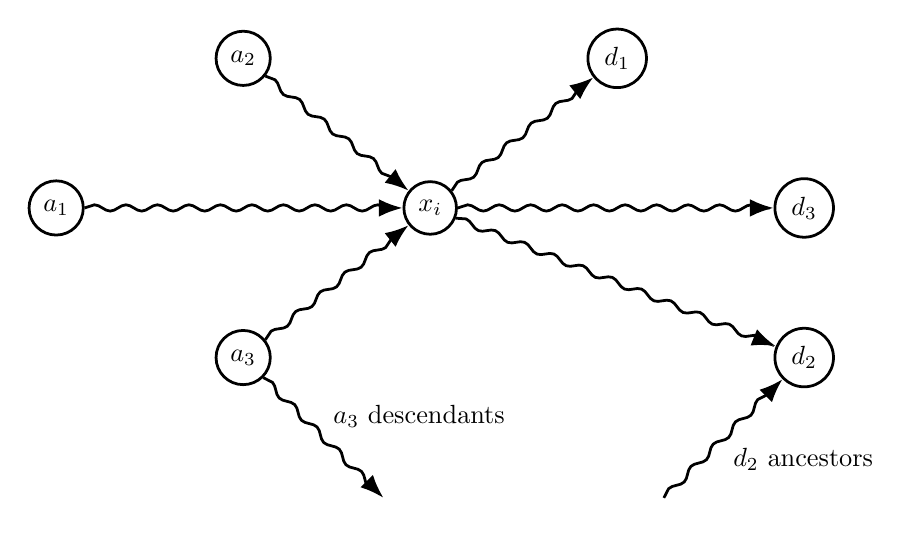
\begin{tikzpicture}[scale=.95, transform shape]
        % ---- NODOS ----
        \node[nodo] (a1) at (0, 0) {$a_1$};
        \node[nodo] (a2) at (2.5, 2) {$a_2$};
        \node[nodo] (a3) at (2.5, -2) {$a_3$};
        \node[nodo] (xi) at (5, 0) {$x_i$};
        \node[nodo] (d_1) at (7.5, 2) {$d_1$};
        \node[nodo] (d_2) at (10, -2) {$d_2$};
        \node[nodo] (d_3) at (10, 0) {$d_3$};
        
        \node[draw=none, fill=none] (hijo_a3) at (4.5, -4) {};
        \node[draw=none, fill=none] (hijo_d2) at (8, -4) {};

        % ---- ARISTAS ----
        \path [->] (a1) edge[arista, decorate, decoration={snake, amplitude=.4mm, 
        segment length=4mm, post length=1mm}]  (xi);
        \path [->] (a2) edge[arista, decorate, decoration={snake, amplitude=.4mm, segment length=4mm, post length=1mm}]  (xi);
        \path [->] (a3) edge[arista, decorate, decoration={snake, amplitude=.4mm, segment length=4mm, post length=1mm}]  (xi);
         \path [->] (xi) edge[arista, decorate, decoration={snake, amplitude=.4mm, segment length=4mm, post length=1mm}]  (d_1);
         \path [->] (xi) edge[arista, decorate, decoration={snake, amplitude=.4mm, segment length=4mm, post length=1mm}]  (d_2);
         \path [->] (xi) edge[arista, decorate, decoration={snake, amplitude=.4mm, segment length=4mm, post length=1mm}]  (d_3);
         \path [->] (a3) edge[arista, decorate, decoration={snake, amplitude=.4mm, segment length=4mm, post length=1mm}] node[above right] {$a_3$ descendants} (hijo_a3);
         \path [->] (hijo_d2) edge[arista, decorate, decoration={snake, amplitude=.4mm, segment length=4mm, post length=1mm}] node[below right] {$d_2$ ancestors} (d_2);

    \end{tikzpicture}
    \caption{When fixing a node $x_i$ we can split the rest of the nodes in three groups: \textit{ancestors} (every node able to reach $x_i$), \textit{descendants} (every node reachable from $x_i$) and those \textit{unrelated} with $x_i$.}
\end{figure}
For every topological order $\toOr$ we know that every $a \in A$ appears before $x_i$, $\toOr(a) < \toOr(x_i)$, and that every $d \in D$ appears after,$\toOr(x_i) < \toOr(d)$. If they were the only nodes to take into account, then \numTopo($G$)= \#$A! \cdot \#D!$, that's the permutations of $A$ times the permutation of $D$. Also, all of them will  be in the same equivalence class, because the order of the attributes in each permutation $\toOr^1, \toOr^2$ won't affect the result of evaluating $\charactheristicFunction$ ($\charactheristicFunction(\toOr^1) = \charactheristicFunction(\toOr^2)$). They will have the same fixed attributes before $x_i$, $A$,  and the same after $x_i$, $D$. That gives us this formula,  $$\sum_{\toOr \in \topo(G)} [\charactheristicFunction(\toOr_{<i} \cup \{x_i\}) - \charactheristicFunction(\toOr_{<i})] = ( \charactheristicFunction(\toOr_{<i} \cup \{x_i\}) - \charactheristicFunction(\toOr_{<i}) ) * \#A! \cdot \#D!$$ (for any $\toOr \in \topo(G))$, because all the evaluations of $\charactheristicFunction$ give the same result for any $\toOr$. That means that we can reduce the number of times that we will evaluate $\charactheristicFunction$.

But in the DAG $G$ we have nodes that aren't descendants or ancestors  of $x_i$,they will be $U$, the \emph{unrelated nodes}. There can be multiple equivalence classes, and we will need to discover all of them and their sizes. With that information, we can calculate the $ASV$: $$\assym_{M,e,\Pr}(x_i) = \sum_{\toOr \in \topo(G)} \charactheristicFunction(\toOr_{<i} \cup \{x_i\}) - \charactheristicFunction(\toOr_{<i}) = \heuristicASVFormula$$

If we can calculate the number and size of the equivalence classes in an efficient manner then we can calculate the $ASV$ value. For the size of the equivalence classes, we want to calculate the number of topological orders of a certain DAG. 

\subsubsection{Number of topological orders of a DAG} %¿Or polytree?
\label{Number Of Toposorts}

We are going to define a formula to calculate the number of topological orders of a DAG. Let's start with the most basic DAG $D$, a graph with $n+1$ nodes and no edges. 

\begin{figure}[ht]
\centering 
 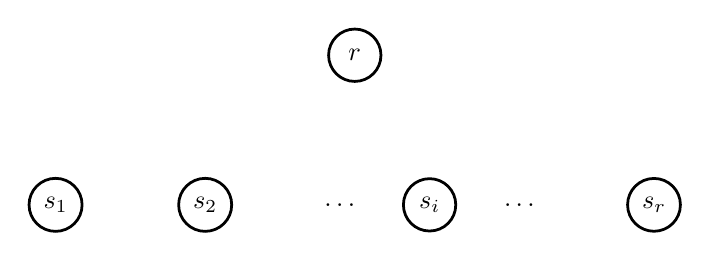
\begin{tikzpicture}[scale=.95, transform shape]

        % ---- NODOS ----
        \node[nodo] (r) at (0, 0) {$r$};
        \node[nodo] (s1) at (-4, -2) {$s_1$};
        \node[nodo] (s2) at (-2, -2) {$s_2$};
        \node[nodo] (si) at (1, -2) {$s_i$};
        \node[nodo] (sn-1) at (4, -2) {$s_{r}$};
        
        \node[draw=none, fill=none] (dots) at (-0.2, -2) {$\ldots$}; % Ellipsis
        \node[draw=none, fill=none] (dots) at (2.2, -2) {$\ldots$}; % Ellipsis
        
        % \node[draw=none, fill=none] (hijo_a3) at (4.5, -4) {};
        % \node[draw=none, fill=none] (hijo_d2) at (8, -4) {};
        
    \end{tikzpicture}
\end{figure}

In this case the number of topological orders of $D$ is $n!$, because the nodes don't have any edges between them, so there are no restrictions. Now let's add some edges to $D$ so that it becomes a tree and let's imagine that each node $s_j$ has it's own subtree. 

\begin{figure}[ht]
\centering 
 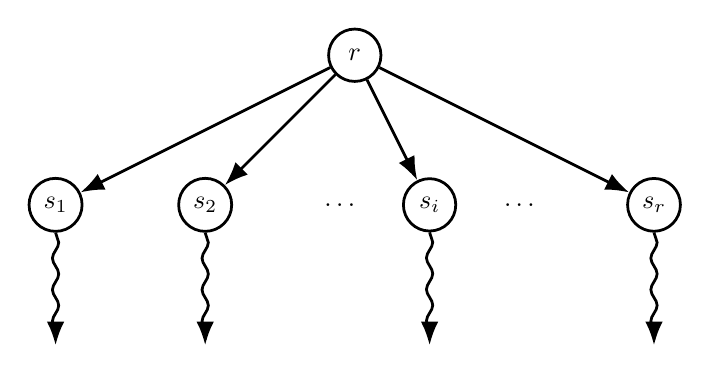
\begin{tikzpicture}[scale=.95, transform shape]

        % ---- NODOS ----
        \node[nodo] (r) at (0, 0) {$r$};
        \node[nodo] (s1) at (-4, -2) {$s_1$};
        \node[nodo] (s2) at (-2, -2) {$s_2$};
        \node[nodo] (si) at (1, -2) {$s_i$};
        \node[nodo] (sn-1) at (4, -2) {$s_{r}$};
        
        \node[draw=none, fill=none] (dots) at (-0.2, -2) {$\ldots$}; % Ellipsis
        \node[draw=none, fill=none] (dots) at (2.2, -2) {$\ldots$}; % Ellipsis
        
        \node[draw=none, fill=none] (h1) at (-4, -4) {};
        \node[draw=none, fill=none] (h2) at (-2, -4) {};
        \node[draw=none, fill=none] (hi) at (1, -4) {};
        \node[draw=none, fill=none] (hn-1) at (4, -4) {};


         \path [->] (r) edge[arista]  (s1);
         \path [->] (r) edge[arista]  (s2);
         \path [->] (r) edge[arista]  (si);
         \path [->] (r) edge[arista]  (sn-1);

        \path [->] (s1) edge[arista,  decorate, decoration={snake, amplitude=.4mm, segment length=4mm, post length=1mm}]  (h1);
         \path [->] (s2) edge[arista,  decorate, decoration={snake, amplitude=.4mm, segment length=4mm, post length=1mm}]  (h2);
         \path [->] (si) edge[arista,  decorate, decoration={snake, amplitude=.4mm, segment length=4mm, post length=1mm}]  (hi);
         \path [->] (sn-1) edge[arista,  decorate, decoration={snake, amplitude=.4mm, segment length=4mm, post length=1mm}]  (hn-1);
    \end{tikzpicture}
\end{figure}

% Misma idea que en https://cs.stackexchange.com/questions/12713/find-the-number-of-topological-sorts-in-a-tree
Here the formula is recursive, and it depends on each of the subtrees of $D$. Now we have $n+1$ nodes, and the subtrees $t_1, \dots, t_r$ of the children $s_j$, have $k_1, \dots, k_r$ nodes respectively (with $n= k_1 + \dots + k_r$). Now let $\numTopo(r)$ be the number of topological orders of the tree $D$ with root $r$. Then the formula we have is: 

$$\numTopo(t) =  \binom{n}{k_1, k_2, \ldots, k_r} \prod_{i=1}^{n} \numTopo(t_i)$$

You can combine the topological orders of each child by selecting which position you are going to assign to each of them, the number of different assignments that you can do in $n$ positions with $r$ sets of $k_i$ elements each is: $ \binom{n}{k_1, k_2, \ldots, k_r}= \frac{n!}{k_1! k_2! \ldots, k_r!}$. Now for all of those assignments you can use any of the topological orders of each subtree, that's the $\prod_{i=1}^{n} \numTopo(t_i)$.

We could try to add more edges to our graph $D$, for example an edge $(r,d)$ between $r$ and one of it's descendants $d$.

\begin{figure}[ht]
\centering 
 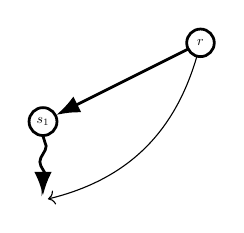
\begin{tikzpicture}[scale=.5, transform shape]

        % ---- NODOS ----
        \node[nodo] (r) at (0, 0) {$r$};
        \node[nodo] (s1) at (-4, -2) {$s_1$};
       
        \node[draw=none, fill=none] (h1) at (-4, -4) {};

         \path [->] (r) edge[arista]  (s1);
         \draw[->] (r) to[bend left] (h1);


        \path [->] (s1) edge[arista,  decorate, decoration={snake, amplitude=.4mm, segment length=4mm, post length=1mm}]  (h1);

    \end{tikzpicture}
\end{figure}

But it would stop being a polytree, because it would introduce a cycle in the undirected graph. Something that we can add are multiple roots $r_1, \dots, r_l$ in our graph, that would still be a polytree. And we can calculate the \numTopo \ of it by adding a root $r_0$ that is connected to all of them and use the same formula as if it was a tree. 

\begin{figure}[ht]
\centering 
 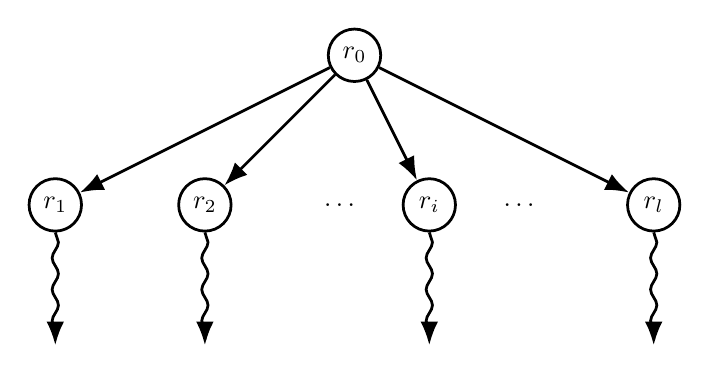
\begin{tikzpicture}[scale=.95, transform shape]

        % ---- NODOS ----
        \node[nodo] (r) at (0, 0) {$r_0$};
        \node[nodo] (s1) at (-4, -2) {$r_1$};
        \node[nodo] (s2) at (-2, -2) {$r_2$};
        \node[nodo] (si) at (1, -2) {$r_i$};
        \node[nodo] (sn-1) at (4, -2) {$r_{l}$};
        
        \node[draw=none, fill=none] (dots) at (-0.2, -2) {$\ldots$}; % Ellipsis
        \node[draw=none, fill=none] (dots) at (2.2, -2) {$\ldots$}; % Ellipsis
        
        \node[draw=none, fill=none] (h1) at (-4, -4) {};
        \node[draw=none, fill=none] (h2) at (-2, -4) {};
        \node[draw=none, fill=none] (hi) at (1, -4) {};
        \node[draw=none, fill=none] (hn-1) at (4, -4) {};


         \path [->] (r) edge[arista]  (s1);
         \path [->] (r) edge[arista]  (s2);
         \path [->] (r) edge[arista]  (si);
         \path [->] (r) edge[arista]  (sn-1);

        \path [->] (s1) edge[arista,  decorate, decoration={snake, amplitude=.4mm, segment length=4mm, post length=1mm}]  (h1);
         \path [->] (s2) edge[arista,  decorate, decoration={snake, amplitude=.4mm, segment length=4mm, post length=1mm}]  (h2);
         \path [->] (si) edge[arista,  decorate, decoration={snake, amplitude=.4mm, segment length=4mm, post length=1mm}]  (hi);
         \path [->] (sn-1) edge[arista,  decorate, decoration={snake, amplitude=.4mm, segment length=4mm, post length=1mm}]  (hn-1);
    \end{tikzpicture}
\end{figure}

If we have multiple roots, then it could happen that they share some common descendants. But if two roots $r_i$ and $r_j$ share two or more descendants $d_1$ and $d_2$ then they would have a cycle in their undirected graph, between those two roots. That implies that two roots can only share one descendant at most. For example, this would be a valid polytree. 

\begin{figure}[ht]
\centering 
 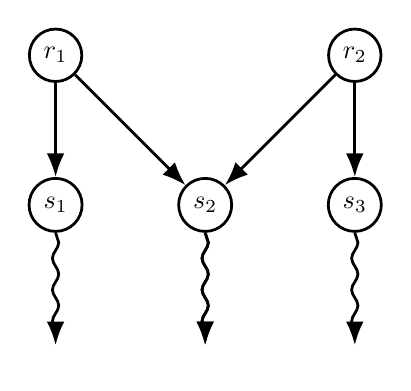
\begin{tikzpicture}[scale=.95, transform shape]

        % ---- NODOS ----
        \node[nodo] (r1) at (-2,0) {$r_1$};

        \node[nodo] (r2) at  (2,0) {$r_2$};
        
        \node[nodo] (s1) at (-2,-2) {$s_1$};
        \node[nodo] (s2) at (0,-2) {$s_2$};
        \node[nodo] (s3) at (2,-2) {$s_3$};
        

        \node[draw=none, fill=none] (h1) at (-2, -4) {};
        \node[draw=none, fill=none] (h2) at (0, -4) {};
        \node[draw=none, fill=none] (h3) at (2, -4) {};


         \path [->] (r1) edge[arista]  (s1);
         \path [->] (r1) edge[arista]  (s2);
         \path [->] (r2) edge[arista]  (s2);
         \path [->] (r2) edge[arista]  (s3);

        \path [->] (s1) edge[arista,  decorate, decoration={snake, amplitude=.4mm, segment length=4mm, post length=1mm}] (h1);
         \path [->] (s2) edge[arista,  decorate, decoration={snake, amplitude=.4mm, segment length=4mm, post length=1mm}]  (h2);
         \path [->] (s3) edge[arista,  decorate, decoration={snake, amplitude=.4mm, segment length=4mm, post length=1mm}]  (h3);


        \path [->] (s2) edge[arista,  decorate, decoration={snake, amplitude=.4mm, segment length=4mm, post length=1mm}]  (h2);
    \end{tikzpicture}
\end{figure}

%TODO: Resolver este caso!!! Consultas a Pablo que dice que es izi pizi esto

In this case, we cannot use the same formula as the tree, cause there is some overlapping between the subtrees of $r_1$ and $r_2$. We know that there cannot be any edges between the subtrees of $s_1$, $s_2$ and $s_2$, $s_3$ because that would create a cycle. \emph{But we could not determine a closed formula for this scenario. }

The formula that we have then is: $$\numTopo(t) =  \binom{n}{k_1, k_2, \ldots, k_r} \prod_{i=1}^{n} \numTopo(t_i)$$
Analyzing this formula, we can see that:

\begin{itemize}
    \item If we have big subtrees, then the number of topological orders can be something closer to polynomial in $n$ (the number of nodes). 
    \item If you have a small enough maximum out degree $m$, then you will know that for each level, the biggest $k$ (size of the subtree) will be bounded by $\frac{n}{m}$.
    \item  If you have a tree that is composed of multiple paths without a great length, then the number of topological orders could be tractable. 
\end{itemize}

\begin{comment}
    $TODO: Do this proof$
    \begin{lemma}\label{lemma:pr_equals_prprime}
    For any tree $T$ and it's root $n$, where $l$ is the number of leaves of the tree and $h$ is its height. Then for the formula: 
    \[
    \numTopo(n) = 
    \begin{cases} 
    1 & \text{if $n$ is a leaf} \\
    \binom{n}{k_1, k_2, \ldots, k_r} \prod_{i=1}^{n} \numTopo(t_i) & \text{oc.}
    \end{cases}
    \]

    We have the bound $\numTopo(n) \leq (2+h)^l + 1$
      
\end{lemma}

    \begin{proof}
        We want to prove that $\numEqCl(n) \leq (2+h)^l + 1$. This applies to any tree $T$ and it's root $n$, where $l$ is the number of leaves of the tree and $h$ is its height.

        We have to prove this for the two cases that the formula presents. 

        \textbf{Case 1: $n$ is a leaf}
        If $n$ is a leaf, then it has height 0, and it's a number of leaves is 1. That leaves us with  $\numEqCl(n) = 2\leq  3 = (2+0)^1 + 1$. 

        \textbf{Case 2: $n$ has children}

        Our \textit{inductive hypothesis} is that for each subtree $T_h$ that has a child $c$ of $n$ as a root, our formula stands. That means that $\forall c \in children(n), \numEqCl(c) \leq (2+ h_c)^{l_c} + 1$. With this in mind let's start
        \begin{align}\label{eq:pr_equals_prprime}
            \numEqCl(n)  &= \prod_{c \in children(n)} \numEqCl(c) + 1 \\
            & \leq (applying \ the \ IH) \prod_{c \in children(n)} ((2+ h_c)^{l_c} + 1) + 1 \\
            & \leq \prod_{c \in children(n)} (2+ h_c)^{l_c} + 1 \\
            & \leq (h>h_c) \prod_{c \in children(n)} (2+ h)^{l_c} + 1 \\
            & = (2+ h)^{\sum_{c \in children(n)} l_c} + 1 \\
            & = (\sum_{c \in children(n)} l_c = l) \ (2+ h)^l + 1 \\
            & = (2+ h)^l + 1 \\
        \end{align}

    That's how we conclude that our formula has an upper bound of $(2+ h)^l + 1$. 
    \end{proof}
\end{comment}

 
\subsubsection{Number of equivalence classes of a DAG} %¿Or polytree?

We have defined a formula to calculate the size of each equivalence class, now we need one to calculate the number of equivalence classes. As it was mentioned in section \ref{heuristic_asv_section}, what we will be looking at are the \emph{unrelated nodes}, $U$, and the relationships between them. These are the nodes that aren't descendants or ancestors of $x_i$ (the feature for which we are calculating $ASV$). Let's start with the case of calculating the number of equivalence classes $\eqCl$ for a tree, with feature $x_i$.

\begin{figure}[ht]
\centering 
 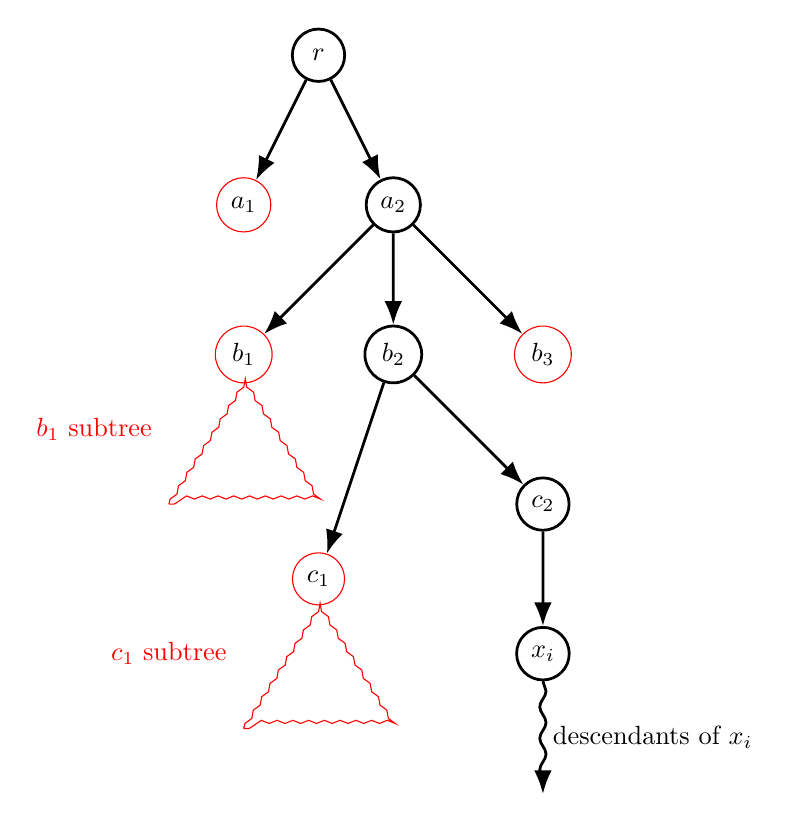
\begin{tikzpicture}[scale=.95, transform shape, 
    unrelated/.style={circle, draw=red},
    wiggly/.style={decorate, decoration={snake, amplitude=.2mm, segment length=2mm}}  % Define wiggly line style
    ]
        
        
        % ---- NODOS ----
        \node[nodo] (r) at (0, 0) {$r$};
        \node[unrelated] (a1) at (-1, -2) {$a_1$};
        \node[nodo] (a2) at (1, -2) {$a_2$};

        \node[unrelated] (b1) at (-1, -4) {$b_1$};
        \node[nodo] (b2) at (1, -4) {$b_2$};
        \node[unrelated] (b3) at (3, -4) {$b_3$};

        \node[unrelated] (c1) at (0, -7) {$c_1$};
        \node[nodo] (c2) at (3, -6) {$c_2$};

        \node[nodo] (xi) at (3, -8) {$x_i$};


        
        \node[draw=none, fill=none] (hi) at (3, -10) {};


         \path [->] (r) edge[arista]  (a1);
         \path [->] (r) edge[arista]  (a2);

         \path [->] (a2) edge[arista]  (b1);
         \path [->] (a2) edge[arista]  (b2);
         \path [->] (a2) edge[arista]  (b3);

         \path [->] (b2) edge[arista]  (c1);
         \path [->] (b2) edge[arista]  (c2);

         \path [->] (c2) edge[arista]  (xi);


        \node[text=red] at (-2, -8) {$c_1$ subtree}; 
        \draw[red, wiggly] (-1, -9) -- (0,-7.4) -- (1, -9) -- cycle;  % Draw the triangle

        \node[text=red] at (-3, -5) {$b_1$ subtree}; 
        \draw[red, wiggly] (-2, -6) -- (-1,-4.4) -- (0, -6) -- cycle;  % Draw the triangle
        
         \path [->] (xi) edge[arista,  decorate, decoration={snake, amplitude=.4mm, segment length=4mm, post length=1mm}] node[right] {descendants of $x_i$} (hi);
    \end{tikzpicture}
\end{figure}

In this case, the nodes that we care about are the ones in red. Because the descendants of $x_i$ will always be to the right of $x_i$ in the topological order and it's ancestors will appear before, so they won't define new equivalence classes. If there wasn't any relation between the \emph{unrelated} nodes then, the number of classes would be $2^{|U|}$. Because if you have a topological order $\toOr$, then you know that $\toOr =  \left[ ancestors, \dots x_i , \dots , descendants  \right] $ it will be something similar to this. Then you just need to define where to insert the $U$ nodes, but if they have no relationships between them then you each of them can be put to the left or to the right of $x_i$, defining a new equivalence class. 
%TODO : Buscar una forma mejor de decir esto

What happens when some of this unrelated nodes have descendants? Let's calculate the number of equivalence classes for one of the subtrees. For example, this could be the $b_1$ subtree in the previous example. 

\begin{figure}[ht]
\centering 
 \begin{tikzpicture}[scale=.95, transform shape, 
    unrelated/.style={circle, draw=red},
    ]
        
        
        % ---- NODOS ----
        \node[unrelated] (b1) at (0, 0) {$b1$};
        \node[unrelated] (11) at (-1, -2) {$1_1$};
        \node[unrelated] (12) at (1, -2) {$1_2$};

        \node[unrelated] (21) at (-1, -4) {$2_1$};
        \node[unrelated] (22) at (1, -4) {$2_2$};
        \node[unrelated] (23) at (3, -4) {$2_3$};

         \path [->] (r) edge[arista, draw=red]  (a1);
         \path [->] (r) edge[arista, draw=red]  (a2);

         \path [->] (a1) edge[arista, draw=red]  (21);
         \path [->] (a2) edge[arista, draw=red]  (b2);
         \path [->] (a2) edge[arista, draw=red]  (b3);

    \end{tikzpicture}
\end{figure}

We want to calculate the number of equivalence classes of the tree rooted in $b1$, $\numEqCl(b_1)$. For $b_1$ we have two options, it can be positioned to the right or to the left of $x_i$ in the topological order $\toOr$. If it's positioned to the right, then all of its descendants will be positioned to the right two, because it's a toposort (topological order). 
%TODO: Reemplazar los topological order por toposort.
%TODO: Usar otro conector que no sea because, cause, that means. 
So our formula would be $$\numEqCl(b_1) = \numEqCl(b_1) \land \toOr(b_1) > \toOr(x_i) + \numEqCl(b_1) \land \toOr(b_1) < \toOr(x_i)  = 1 + \numEqCl(b_1) \land \toOr(b_1) < \toOr(x_i) $$

\santi{Esta suma está rara.}
\echu{Esta formula es una poronga, hay que modificarla y dejar algo más coherente. }

Now if $b_1$ is positioned on the left of $x_i$ then there is no restriction for its children and their subtrees, and we can apply the same process. Then for each $\eqCl$ that we obtain in its subtrees we can combine them, cause they won't be restricted. In probability, that means multiplying the result that we obtain for each tree. We have to also take into account the case where the node has no children, there we can have two equivalence classes, taking into account the left and right possibilities. That's how we obtain this formula: 

\label{formula:number_of_equiv_classes}
\[
\numEqCl(n) = 
\begin{cases} 
2 & \text{if $n$ is a leaf} \\
\prod_{c \in children(n)} \numEqCl(c) + 1 & \text{oc.}
\end{cases}
\]

This formula can also be used to calculate the equivalence classes of all the \emph{unrelated} nodes in the previous example, we can use a similar strategy than the one for calculating the toposorts. We create a node $r_0$ and connect it to the roots of all the subtrees of the unrelated nodes, and then calculate $\numEqCl(r_0)$ using the formula previously defined. 

\begin{figure}[ht]
\centering 
     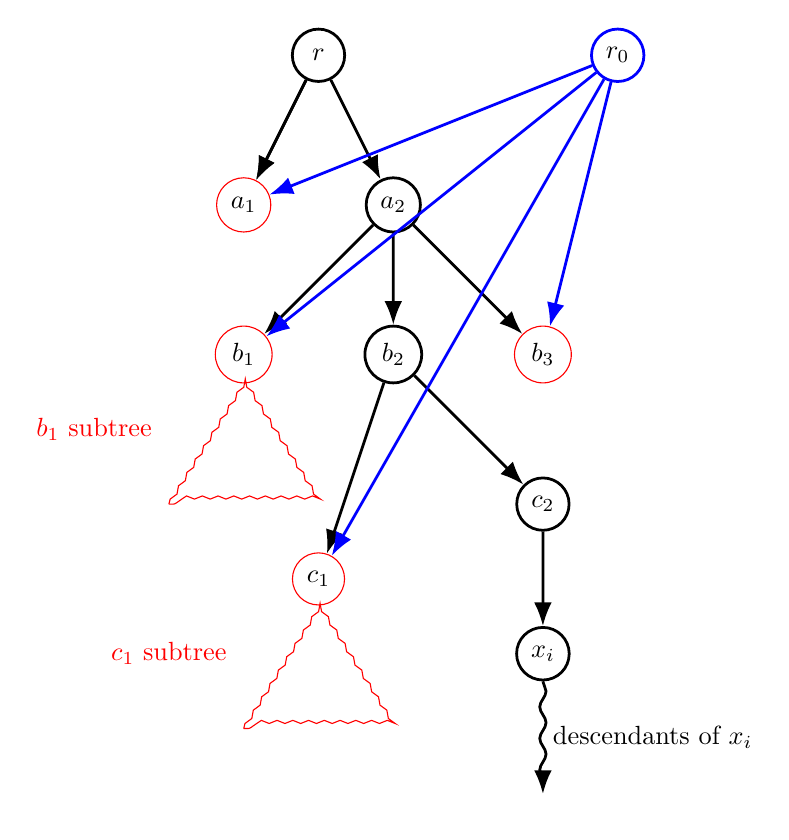
\begin{tikzpicture}[scale=.95, transform shape, 
    unrelated/.style={circle, draw=red},
    wiggly/.style={decorate, decoration={snake, amplitude=.2mm, segment length=2mm}}  % Define wiggly line style
    ]
        
        
        % ---- NODOS ----
        \node[nodo] (r) at (0, 0) {$r$};
        \node[nodo, draw=blue] (r0) at (4, 0) {$r_0$};
        \node[unrelated] (a1) at (-1, -2) {$a_1$};
        \node[nodo] (a2) at (1, -2) {$a_2$};

        \node[unrelated] (b1) at (-1, -4) {$b_1$};
        \node[nodo] (b2) at (1, -4) {$b_2$};
        \node[unrelated] (b3) at (3, -4) {$b_3$};

        \node[unrelated] (c1) at (0, -7) {$c_1$};
        \node[nodo] (c2) at (3, -6) {$c_2$};

        \node[nodo] (xi) at (3, -8) {$x_i$};


        
        \node[draw=none, fill=none] (hi) at (3, -10) {};


         \path [->] (r) edge[arista]  (a1);
         \path [->] (r) edge[arista]  (a2);

         \path [->] (a2) edge[arista]  (b1);
         \path [->] (a2) edge[arista]  (b2);
         \path [->] (a2) edge[arista]  (b3);

         \path [->] (b2) edge[arista]  (c1);
         \path [->] (b2) edge[arista]  (c2);

         \path [->] (c2) edge[arista]  (xi);

        \path [->] (r) edge[arista]  (a1);
        \path [->] (r0) edge[arista, draw=blue]  (a1);
        \path [->] (r0) edge[arista, draw=blue]  (b1);
        \path [->] (r0) edge[arista, draw=blue]  (b3);
        \path [->] (r0) edge[arista, draw=blue]  (c1);
        
        \node[text=red] at (-2, -8) {$c_1$ subtree}; 
        \draw[red, wiggly] (-1, -9) -- (0,-7.4) -- (1, -9) -- cycle;  % Draw the triangle

        \node[text=red] at (-3, -5) {$b_1$ subtree}; 
        \draw[red, wiggly] (-2, -6) -- (-1,-4.4) -- (0, -6) -- cycle;  % Draw the triangle
        
         \path [->] (xi) edge[arista,  decorate, decoration={snake, amplitude=.4mm, segment length=4mm, post length=1mm}] node[right] {descendants of $x_i$} (hi);
    \end{tikzpicture}
\end{figure}

There is one case that we are not taking into consideration, and that's when the unrelated nodes have ancestors. But that's the same case for which \emph{we could not find an answer} in the counting of the toposorts. In this case it would be easy to fix it, cause you would just need to conect $r_0$ to the new root of the subtree. The problem is if the subtre has multiple roots, then the formula that we defined previously would not be enough, cause it would be counting some scenarios twice. 
%TOOD: Resolver este caso para los ordenes topologicos, así lo podemos hacer para las clases de equivalencia también. 

\paragraph{Bound for the number of equivalence classes}

For the multiple scenarios that we took into consideration, we would want to find a bound for the number of equivalence classes. This formula has an upper bound, and we are going to prove it. 

\begin{lemma}\label{lemma:upper_bound_equivalence_classes}
    For any tree $T$ and it's root $n$, where $l$ is the number of leaves of the tree and $h$ is its height. Then for the formula: 
    \[
    \numEqCl(n) = 
    \begin{cases} 
    2 & \text{if $n$ is a leaf} \\
    \prod_{c \in children(n)} \numEqCl(c) + 1 & \text{oc.}
    \end{cases}
    \]

    We have the bound $\numEqCl(n) \leq (2+h)^l + 1$
      
\end{lemma}

    \begin{proof}
        We want to prove that $\numEqCl(n) \leq (2+h)^l + 1$. This applies to any tree $T$ and it's root $n$, where $l$ is the number of leaves of the tree and $h$ is its height.

        We have to prove this for the two cases that the formula presents. 

        \textbf{Case 1: $n$ is a leaf}
        If $n$ is a leaf, then it has height 0, and it's a number of leaves is 1. That leaves us with  $\numEqCl(n) = 2\leq  3 = (2+0)^1 + 1$. 

        \textbf{Case 2: $n$ has children}

        Our \textit{inductive hypothesis} is that for each subtree $T_h$ that has a child $c$ of $n$ as a root, our formula stands. That means that $\forall c \in children(n), \numEqCl(c) \leq (2+ h_c)^{l_c} + 1$. With this in mind let's start
        \begin{align}\label{eq:pr_equals_prprime}
            \numEqCl(n)  &= \prod_{c \in children(n)} \numEqCl(c) + 1 \\
            & \leq (applying \ the \ IH) \prod_{c \in children(n)} ((2+ h_c)^{l_c} + 1) + 1 \\
            & \leq \prod_{c \in children(n)} (2+ h_c)^{l_c} + 1 \\
            & \leq (h>h_c) \prod_{c \in children(n)} (2+ h)^{l_c} + 1 \\
            & = (2+ h)^{\sum_{c \in children(n)} l_c} + 1 \\
            & = (\sum_{c \in children(n)} l_c = l) \ (2+ h)^l + 1 \\
            & = (2+ h)^l + 1 \\
        \end{align}

    That's how we conclude that our formula has an upper bound of $(2+ h)^l + 1$. 
    \end{proof}
%\sidesergio{Obs: si no se van a referenciar líneas, creo que es mejor usar align*}

With this bound, we can see that: 

\begin{itemize}
    \item If the number of leaves is $O(\log n)$ and the height of the tree is $O(1)$ then we can have a number of equivalence classes polynomial in the size of $n$. \santi{Esto lo habíamos hablado una vez. SI tenés $O(\log n)$ hojas no podés tener altura $O(1)$ (porque multiplicar hojas por pisos da una cota superior a la cantidad de nodos).}
    \item We want to have the minimum amount of leaves possible, that means that we want to have a small out degree from each vertex, the same that happens for the toposort. 
    \item It's better to have a bigger height than a bigger out degree with a lot of branching. 
\end{itemize}

%TOOD: Pensar más cosas que podemos inferir de la misma


\subsection{Bayesian Networks}

%When we are calculating the Assymetric Shapley Value we need a casualty DAG $G$ that defines the relationship between the features and a probability distribution $Pr$ function. In our case we will be using Bayesian Networks as $G$ and $Pr$, it will define the probability of each feature and also the casualty graph. A Bayesian Network $B$ is a $DAG$, where each node represents a different variable and the arcs represent the conditional dependencies between them. For example, if we have the arc $A \longrightarrow B$ then this represents that the variable $B$ is dependent on $A$, and that is quantified using the conditional probability $P(B|A)$. A node can have multiple parent's, so the probability of the node will be defined in a \emph{Conditional Probability Table} (CPT), the probability of the node taking on a particular value, given the values of its parent node. With that, we can define a Bayesian Network as:

\begin{definition}
A Bayesian Network consists of the following:

\begin{itemize}
    \item A set of variables and a set of directed edges between variables, where each variable has a finite set of mutually exclusive states.
    \item The variables together with the directed edges form an acyclic directed graph (traditionally abbreviated DAG); a directed graph is acyclic if there is no directed path $A_1 \rightarrow \dots \rightarrow A_n$ so that $A_1 = A_n$.
    \item To each variable $A$ with parents $B_1, \dots, B_n$, a conditional probability table (CPT) $P(A \mid B_1, \dots, B_n)$ is attached.
\end{itemize}
    
\end{definition}

\begin{figure}[ht]
    \centering
    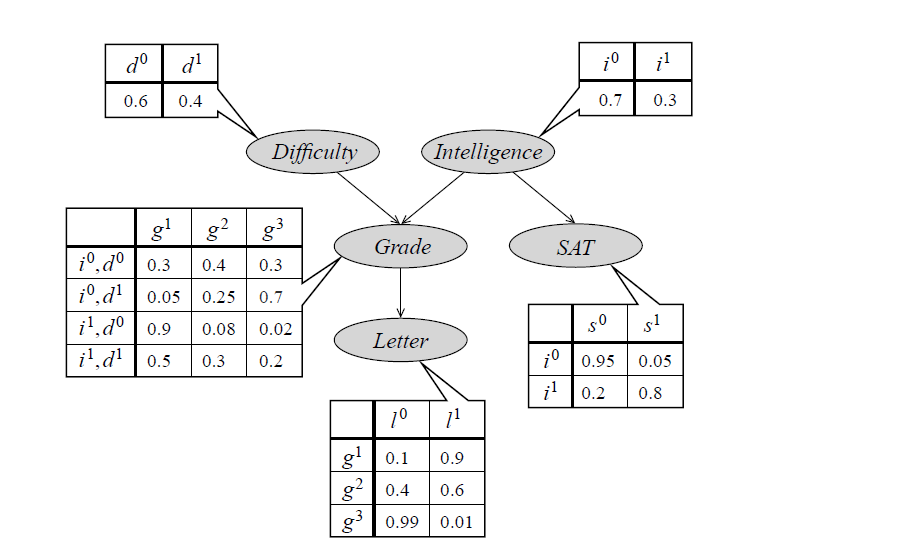
\includegraphics[scale=0.4]{img/bayesianNetworks.png}
    \caption{Bayesian Network for determining a students' intelligence. We can see that each node has a $CPT$ that it's calculated based on it's parent's, here the variables are binary.}
    \label{fig:bayesian_network_example}
\end{figure}

\newpage
 
 This kind of networks help us to simplify the computation of joint probability distributions. One of its most important properties, it's the \emph{chain rule}, it provides a  fundamental structure for understanding how joint probabilities can be decomposed in the context of Bayesian networks. Specifically, it states that if we let \( BN \) be a Bayesian network over a set of variables \( \{A_1, \dots, A_n\} \), then \( BN \) specifies a unique joint probability distribution \( P(U) \), where \( U = \{A_1, \dots, A_n\} \), that can be expressed as the product of all CPT's specified in \( BN \). Mathematically, it is represented as:
\[
P(U) = \prod_{i=1}^{n} P(A_i \mid \text{pa}(A_i))
\]
where \( \text{pa}(A_i) \) denotes the parents of \( A_i \) in the Bayesian network. This rule is essential because it simplifies the computation of the joint probability distribution of a complex network by breaking it down into simpler, local dependencies between a node and its direct predecessors. Thus, the chain rule encapsulates the essence of Bayesian networks, where local dependencies aggregate to define a global distribution, facilitating both the learning and inference processes within these networks.

%Hablar acerca de las operaciones que se pueden hacer, inferencia e instanciar variables + sus complejidades según los tipos de redes con los que uno trabaja

Furthermore, Bayesian networks facilitate a variety of computational operations crucial for probabilistic inference. One of the primary operations is \textbf{inference}, which involves computing the prior distribution for some variable. That means, calculating $Pr(A)$, being $A$ a node in the network. This process is often referred to as \emph{querying} the network. The complexity of inference depends on the network's structure, for polytree-shaped, also known as \emph{singly connected},  networks, the complexity is polynomial on the size of the network variables. \cite{pearl1986bayesianInference}. 

Another critical operation is \textbf{variable instantiation}, which involves setting the values of certain variables and observing the effects on the probabilities of other variables. In this case, we are introducing evidence into the network, which is the posterior distribution. An algorithm that we can use to perform these operations is the \emph{Variable Elimination}.\cite{Darwiche_2009} This algorithm can also run in polynomial time for polytree-shaped networks. That means that these two operations, inference and variable instantiation, can be done in a tractable manner for polytrees. 

%Encontre una cota acá, pero no pude encontrar la fuente de donde la sacan. https://www.ime.usp.br/~ddm/courses/mac6916/varelim/#computational-complexity. La cota es O((m+n)*c^(w+1)), siendo c la cardinalidad máxima de alguna de las variables (2 en nuestro caso) y w es la "induced-width of the elimination ordering plus one.". Que en el caso de polytrees, cómo podemos elegir un orden de eliminación óptimo, w está acotado por el tree width. 

%El tree width de un polytree es igual a la máxima cantidad de padres de un nodo, por lo que acotar el grado de entrada de cada nodo nos da una cota para la treeWidth. 
%Revisar mejor de acá https://www.cs.toronto.edu/~hojjat/384f06/Lectures/Lecture17-4up.pdf

%TODO: ¿Hablar más en detalle del algoritmo, del tree-width y de cómo surge esta cota?

%https://cse.hkust.edu.hk/~lzhang/paper/pspdf/canai94.pdf Acá se introdujo el algoritmo de Variable Elimination 

\newpage

%TODO: Hablar de cómo lo nuestro solo funciona para trees actualmente entonces cómo podemos pasar nuestra red bayesiana a un decision tree. 

\begin{comment}
    Quiero remover algunos ejes de la red bayesiana para que me quede un árbol.
Heurística para ver que ejes remover:
¿El eje que me genere un ciclo + genere una menor divergencia entre las distribuciones marginalizadas?
La idea sería fijarse que distribuciones me quedan al removerlo, luego comparar cuáles son las que divergen menos entre sí (criterio KL por ejemplo) y elegir ese eje. 
\end{comment}

\subsubsection{Mean prediction in Decision Trees}

Decision Trees are widely utilized in Artificial Intelligence (AI) for their ability to make predictions and classifications based on features from input data.By breaking down decisions into a series of straightforward questions and answers, decision trees allow users to understand the reasoning behind AI predictions, contributing to transparency in complex systems.

The primary components of a decision tree include nodes, branches, and leaves. Each internal node represents a "condition" based on input features, which bifurcates the data into branches according to their answers. Leaves represent the final outcomes, providing the decision or prediction. There is a direct relationship between the tractability of the \emph{mean} of a model and the $ASV$ \santi{SV?} when the distribution is a \emph{fully factorized} one. So we wanted to see if the calculation of the mean was tractable for decision trees with Bayesian networks distributions, that's how we found this algorithm. \\

%TODO: Redactarlo mejor

For this algorithm, we are going to be working with decision trees, and the features in the tree will be binary. Each node determines a value for one feature $X_i$, with the left child being the case where $X_i=0$ and the right one. They will be a set $X$, and their probability distribution will be a Bayesian network $B$. Then $Pr_B(X_i = k)$ is the probability that the feature $i$ is $k$ given the Bayesian network $B$. And $B_{X_i=k}$ is the Bayesian network $B$ with the feature $i$ instantiated in $k$. 

%TODO: Redactar mejor lo del decision tree binario. 

%TODO: Definimos que nuestra variable a predecir no puede estar en el grafo causal, que no tiene mucho sentido nuestro algoritmo si ese es el caso. Por lo que definimos remover ese feature de nuestra red causal. Agregar esto

%TODO: Hablar de esta operación -> Implementar la operación en las redes bayesianas de <= + probar de calcular el promedio en una red más grande cómo CHILD

\begin{algorithm}
\caption{Mean for Binary Decision Tree}
\begin{algorithmic}[1]
\Function{Mean}{$node$, $B$, $pathCondition$, $evidence$}
    \If{$n$.isLeaf}
        \State \Return  $Pr_B(pathCondition\ | \ evidence)$ * $node.value$
    \EndIf
    \State $X_i \gets n.feature$
    \State $leftMean \gets$  \Call{Mean}{$node$.left, $B$, $pathCondition \cup \set{X_i=0}, evidence$}
    \State $rigthMean \gets$ \Call{Mean}{$node$.right, $B$, $pathCondition \cup \set{X_i=1}, evidence$} 
    \State \Return  \mbox{$leftMean + rigthMean$}
\EndFunction
\end{algorithmic}
\end{algorithm}

Let's analyze the complexity of this algorithm. The operation $Pr_B(X_i = k | evidence)$ is the inference in a Bayesian Network, that means that it has  polynomial time complexity. That implies that the cost of processing each node is polynomial, so the runtime complexity of this algorithm will be polynomial in the size of the decision tree and the Bayesian network. 

%¿Polinomial en base a que? ¿Aclaro de vuelta todo lo anterior? Siento que estoy diciendo todo el tiempo lo mismo, necesito sinonimos de polinomial. ¿Lo hago más formal?

\begin{figure}[ht]
    \centering
    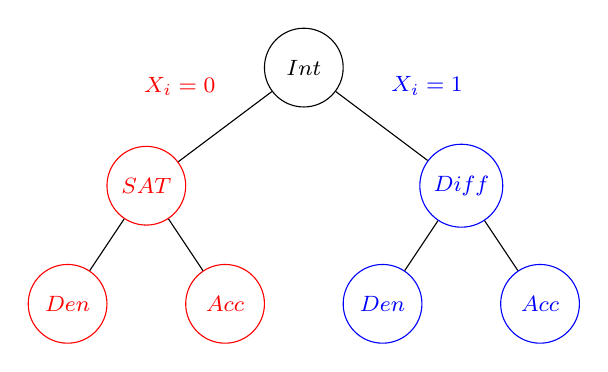
\begin{tikzpicture}[
    level 1/.style={sibling distance=4cm},
    level 2/.style={sibling distance=2cm},
     every node/.style={minimum size=1cm, font=\footnotesize} % Adjust size as needed
]
    \node [circle, draw] {$Int$}
        child {node [circle, draw, red] {$SAT$}
            child {node [circle, draw, red] {$Den$}}
            child {node [circle, draw, red] {$Acc$}}
            edge from parent node[above left] {\textcolor{red}{$X_i=0$}}
        }
        child {node [circle, draw, blue] {$Diff$}
            child {node [circle, draw, blue] {$Den$}}
            child {node [circle, draw, blue] {$Acc$}}
            edge from parent node[above right] {\textcolor{blue}{$X_i=1$}}
        };
    \end{tikzpicture}
    
    \caption{Decision tree for determining if a student will be accepted or denied into a university based on the features of the Bayesian network of figure \ref{fig:bayesian_network_example}.}
    \label{fig:decision_tree_example}
\end{figure}

In figure \ref{fig:decision_tree_example} we have an example of a decision tree. If we run this in the root node of the tree, we will obtain: \echu{Esto ahora no tiene sentido, debería cambiar las cuentas en base a la nueva fórmula}
\begin{align*}
        \Call{Mean}{Int, B} &= Pr_B(Int = 0) * \Call{Mean}{SAT, B_{Int=0}} + Pr_B(Int = 1) * \Call{Mean}{Diff, B_{Int=1}}\\
        &= 0.7 * \Call{Mean}{SAT, B_{Int=0}} +0.3 * \Call{Mean}{Diff, B_{Int=1}} \\
        &= \dots \\
        &= 0.234
    \end{align*}

% Estas cuentas son números cualquiera, tengo que hacerlas y reemplazar con el resultado correcto. 
and we can keep doing this to obtain the result \textbf{calcular el promedio, je}. 

\subsubsection{Time complexity of mean prediction in DT}
% Here we want to compare the naive way (obtaining all the consistent instances vs the mean prediction). 
% We can also compare the time it takes for both and the improvement that the algorithm has versus the naive way. 

\subsubsection{Exact mean prediction computation in Decomposable Circuits}

Can we extend the previous algorithm to work in more general models? We can easily prove an upper bound on model complexity related to the satisfiability problem.

\begin{proposition}
    Let $M$ be a model over entities $\entities(X)$ and $\aDistribution$ a distribution over $\entities(X)$ such that no entity has probability 0. Then, deciding if $\expectancy_{e\sim \aDistribution}[M(e)]$ is positive is equivalent to deciding if $M$ is satisfiable.
\end{proposition}

This does not rule out the tractability of exactly computing the average of models for which the satisfiabilily problem is tractable, such as d-DNNF circuits \cite{arenas2021tractability}. For them, we can prove an intractability result exploiting the correlations that one can impose using the Bayesian Network, which allows us to turn a normal Boolean circuit into a d-DNNF one without altering the average prediction.

\begin{proposition}
    The problem of deciding, given a Bayesian distribution $\aBayesianDistribution$ and a d-DNNF circuit $\aCircuit$ whether $\expectancy_{e \sim \aBayesianDistribution}[\aCircuit(e)] > 0$ is \NPhard{}. Moreover, the results holds for Bayesian Networks which are union of disjoint paths.
\end{proposition}

\begin{proof}
    The problem clearly belongs to $\NP{}$, since we can solve it by guessing an entity $e$ such that $\aCircuit(e)$ and $\Pr[e] > 0$. For the hardness, we reduce \textsc{Circuit-SAT} to our problem.

    Let $\aCircuit$ be a Boolean circuit. Without loss of generality we may assume that it is deterministic (i.e. for each $\vee$ gate the two subcircuits $\aCircuit_1$ and $\aCircuit_2$ cannot be simultaneously satisfied). We are going to design a simple Bayesian distribution such that $\aCircuit$ can be understood also as a decomposable circuit.

    We proceed top-down. Let $\wedge$ be the \textit{and} node closest to the top, and let $\aCircuit_1$ and $\aCircuit_2$ the two subcircuits of this node. In principle, $var(\aCircuit_1) \cap var(\aCircuit_2) \neq \emptyset$. To fix this, let $x_1,\ldots, x_k$ be the variables shared by both subcircuits, and replace the variables $x_1,\ldots,x_k$ from $\aCircuit_2$ with the variables $x_1',\ldots,x_k'$. At the same time, we add to the Bayesian network nodes $x_1,x_1',\ldots,x_k,x_k'$ conditioning that whenever $x_i = 1$ then $x_i'=1$ with probability one, and similarly for the case $x_i = 0$, for all $i$.

    Observe that some entities have probability 0: they are exactly those that pick a different value for $x_i$ and $x_i'$, for some $i$. Therefore, if the expected value of this new circuit is positive then there is an assignment of the original circuit such that it is satisfied.

    To complete the reduction we continue working recursively: at each $\wedge$ gate we detect the shared variables $y_1,\ldots,y_\ell$, change them with variables $y_1',\ldots,y_\ell'$ and add the correlations in the Bayesian network $\aBayesianDistribution$.

    Note that the final structure of the Bayesian network is a set of disjoint paths, over which the inference problem be solved easily.
\end{proof}

\subsection{Approximate mean prediction computation}

Even though exact computation is intractable, approximate calculation is straightforward when considering additive precission.

\begin{proposition}
    Let $\aDistribution$ be any distribution over $\entities(X)$ that can be sampled efficiently, and $\mathcal{F}$ a family of models such that evaluating, given $M \in \mathcal{F}$ and $e \in \entities(X)$, the value $M(e)$,q can be done in polynomial time. Then, there is a \textit{Fully Polynomial-time Approximation Scheme} (FPRAS) for $\expectancy_{e \in \aDistribution}[M(e)]$ under additive error\footnote{I don't think we can achieve multiplicative error, looks like satisfiability.}.
\end{proposition}

\begin{proof}
    Note that $M(e) : \aDistribution \to \{0,1\}$ is a random variable bounded between $0$ and $1$ that can be sampled efficiently, and thus the result follows by considering the Hoeffding's inequality.
\end{proof}


%Tiene sentido poner que no se puede? Y la demo esa de convertir una red no deterministica en una deterministica en polinomial? O alguna otra justificación? 

\section{Algorithm for equivalence classes with forests as causal digraphs}

%We want to obtain the $\assym_{M,e,\Pr}(x_i)$. We also have the causal digraph $G$, which is a forest. We can classify the nodes into ancestors, descendants and unrelated to $x_i$. Now we want to calculate this formula : $$\assym_{M,e,\Pr}(x_i) = \heuristicASVFormula$$

For that, first we will need to calculate all the equivalence classes, one topological order of $G$ that is included in each of them and their respective sizes. We divided this algorithm into two parts, in the first one we obtain the equivalence classes for the unrelated trees and in the second one we merge this classes with the ancestors and ascendants. Here we have our forest example:

\newcommand{\drawUnrelatedTree}[4]{
    \node[unrelated] (#1) at (#2, #3) {#4};
     \pgfmathsetmacro{\x}{#2-2}
     \pgfmathsetmacro{\y}{#3-0.3} 
    \draw[red, wiggly] (#2, \y)
        -- ++(-1,-1.6) 
        -- ++(2,0) 
        -- cycle;
    \node[text=red] at (\x, \y) {#4 subtree};
}

\begin{figure}[H]
    \centering
    \begin{tikzpicture}[scale=.95, transform shape, 
    unrelated/.style={circle, draw=red},
    ancestor/.style={circle, draw=blue},
    wiggly/.style={decorate, decoration={snake, amplitude=.2mm, segment length=2mm}}  % Define wiggly line style
    ]
        \node[text=blue] at (-5, 0) {Ancestors};
        \node[text=teal] at (-5, -0.5) {Descendants};
        \node[text=red] at (-5, -1) {Unrelated};        
        
        % ---- NODOS ----

        \node[ancestor] (a1) at (0, 0) {$a_1$};
        \node[unrelated] (u1) at (-1, -2) {$u_1$};
        \node[ancestor] (a2) at (1, -2) {$a_2$};

        \drawUnrelatedTree{u2}{-1}{-4}{$u_2$}
        \node[ancestor] (a3) at (1, -4) {$a_3$};
        \node[unrelated] (u3) at (3, -4) {$u_3$};

        \drawUnrelatedTree{u4}{0}{-7}{$u_4$}
        \node[ancestor] (a4) at (3, -6) {$a_4$};

        \node[nodo] (xi) at (3, -8) {$x_i$};

        \drawUnrelatedTree{r1}{6}{0}{$u_5$} 
        \drawUnrelatedTree{r2}{10}{0}{$u_6$} 
        
        \node[draw=none, fill=none] (hi) at (3, -10) {};


         \path [->] (a1) edge[arista]  (u1);
         \path [->] (a1) edge[arista]  (a2);

         \path [->] (a2) edge[arista]  (u2);
         \path [->] (a2) edge[arista]  (a3);
         \path [->] (a2) edge[arista]  (u3);

         \path [->] (a3) edge[arista]  (c1);
         \path [->] (a3) edge[arista]  (a4);

         \path [->] (a4) edge[arista]  (xi);      
         \path [->, teal] (xi) edge[arista,  decorate, decoration={snake, amplitude=.4mm, segment length=4mm, post length=1mm}] node[right] {descendants of $x_i$} (hi);
    \end{tikzpicture}
    \caption{Example of a possible causal DAG to calculate the ASV from}
    \label{fig:ASV_forest_example}
\end{figure}



\subsection{Naive formula}

There is also a naive way to calculate this. First, we calculate all the toposorts of the forest using the algorithm proposed in \cite{KNUTH1974153}. After that, we can iterate over the toposorts and assign them to an equivalence class, depending on which unrelated nodes are before $x_i$. After that we will have our classes, a representative for each of them and their classes. The problem here is that we need to calculate explicitly each toposort of $G$, which can be $O(n!)$. 

%TODO : Find a better upper bound, one more tight

\subsection{Equivalence classes for unrelated trees}


First, we need to find the roots of these unrelated trees, we will call this set $UR$. A node $x$ will be a root of an unrelated tree if it's a root and an unrelated node, or if it's only parent is an ancestor of $x_i$. We will represent an equivalence class using a set of which unrelated nodes it has before and after $x_i$, this would be the representation of an $\eqCl = \{ n_t \mid \ n \in V(G) \land t \in  \{ left, right\} \}$. $L(\eqCl)$ and $R(\eqCl)$ will return the number of nodes to the left and to the right in the equivalence class. This algorithm will return a set of tuples with the format $(\eqCl, leftTopos, rightTopos)$. $leftTopos$ being the number of topological orders that we can make with the unrelated nodes before $x_i$ and $rightTopos$ the same but with the ones after.The notation here used is: \\
$n_i$ = $i-th$ child of node $n$, $|n|$ = the number of children of node $n$.
Then we will run this algorithm for each $node \in UR$, here is the algorithm: 

\label{formula:unrelated_equiv_classes}
%  \[
%     \unrEqCl(n) = 
%     \begin{cases} 
%     \set{(\set{n_l}, 1, 1), (\set{n_r},1,1)} & \text{if $n$ is a leaf} \\
%     (\bigcup_{\forall mix \in \unrEqCl(n_1) \times \dots \times \unrEqCl(n_{|n|})} LeftUnion(mix,n)) \cup RightUnion(right,n) & \text{oc.}
%     \end{cases}
% \]


\[
    \unrEqCl(n) = 
    \begin{cases} 
    \set{(\set{n_l}, 1, 1), (\set{n_r},1,1)} & \text{if $n$ is a leaf} \\[1ex]
    \begin{aligned}
    &\left( \bigcup_{\forall mix \in \unrEqCl(n_1) \times \dots \times \unrEqCl(n_{|n|})} \hspace{-6em} LeftUnion(mix,n)\right) \\
    &\cup RightUnion(right,n)
    \end{aligned} & \text{otherwise}
    \end{cases}
\]


%TODO: Dejar más lindo esto, esta feo así

\begin{align*}
&leftUnion(n, ((eqCl_1, lTopo_1, rTopo_1), ...., (eqCl_{|n|}, lTopo_{|n|}, rTopo_{|n|}))) = \\ 
&\left(\bigcup_{j=1}^{|n|} eqCl_j \cup \set{n_l}, \binom{\sum_{i=1}^{|n|} L(eqCl_i)}{L(eqCl_1), \ldots, L(eqCl_{|n|})} \prod_{i=1}^{|n|} lTopo_i, 
\binom{\sum_{i=1}^{|n|} R(eqCl_i)}{R(eqCl_1), \ldots, R(eqCl_{|n|})} \prod_{i=1}^{|n|} rTopo_i \right)
\end{align*}

Here $leftUnion$ represents the union of all the equivalence classes, positioning the node $n$ to the left of $x_i$. We can see the that for calculating the left and right topological orders we use the same formula as in \ref{Number Of Toposorts}. It's the same logic because there are no dependencies between the nodes of the unrelated trees and it's subtrees, so we can mix the toposorts as we like. \\
We also have $rightUnion$, which is the same as $leftUnion$, but in the first tuple it adds $n_r$ instead. It needs to use $right$ because if the node $n$ appears after $x$ \\
$right$ being the product that fulfills that, all of its nodes appear after $x_i$: \\ $right \in \unrEqCl(n_1) \times \dots \times \unrEqCl(n_{|n|}),  \forall (eqCl, \_ , \_) \in right, L(eqCl)=0$ \\

\label{slight_improvement}
There is also a slight improvement implemented, in which we unite some of the unrelated equivalence classes. Let's imagine that we have the results for $\unrEqCl(ur_1)$ and $\unrEqCl(ur_2)$. If $ur_1$ and $ur_2$ have both the same parent or are both roots, then we will unite them. That's because when we are doing the $leftOrders$ calculation, it does not matter if a node comes from either subtree, since they both depend on the same $ancestor$. This optimization will make it so that in $leftOrders$ we have less permutation to calculate. What we do is similar as if in the \ref{fig:ASV_forest_example} we added a virtual node $v$, which is the parent of $u_5$ and $u_6$, and then ran $\unrEqCl$ from it, using only the $leftUnion$ (cause this node does not exist). 

\subsection{Merging of unrelated trees classes with ancestors and descendants}

Now we need to combine the previous classes obtained and merge them with the ancestors and descendants of $x_i$. \\

Foremost, why can't we use the previous formula and just merge them as we were doing before? Let's imagine that we didn't and we just use the $leftUnion$ with the ancestors. The tuple that represents them will be $(\set{ a_l | a \in A}, 1, 1)$, $A$ = $ancestors$. This is because they only have one possible order, and all of them must appear before $x_i$. Now if we used, $leftUnion$ we would be doing this calculation $\binom{|A| + |U|}{|A|}$, that means that we could insert the elements of $A$ between any element of $U$ in the topological order, but that is incorrect! Because in this scenario, there are dependencies between the nodes. In the example \ref{fig:ASV_forest_example} we cannot put $u_1$ before $a_2$ or any of the nodes in the $u_2$ subtree before $a_2$. That means that we need another function to calculate the possible orderings of the nodes that appear before $x_i$ and the ancestors. We are going to call this function $leftOrders$. \\
Now the question is, what do we do with the descendants? Here we are not restricted as we were before with the ancestors, so we can use the same formula that we were using. Because there are no dependencies between the nodes in $D$ and $UR$.\\
Taking that into account, we can finally define the last step. $u_i$ will be root node of the $i-th$ unrelated tree. This is our formula, for calculating all the equivalence classes and their sizes in a forest: 

\label{formula:equiv_classes_sizes}
\[
    \eqClassSizes(G) = 
    \bigcup_{\forall mix \in \unrEqCl(u_1) \times \dots \times \unrEqCl(u_{|UR|})} \left( eqCl(A,D, mix) , \#eqCl(A,D,mix) \right) 
\]

%TODO: Dejar más lindo esto, esta feo así

\begin{align*}
eqClass(A, D, ((eqCl_1, \_ , \_ ), ...., (eqCl_{|UR|}, \_ , \_))) &=  \set{a_l \mid a \in A} \cup \set{d_r \mid d \in D} \cup (\bigcup_{j=1}^{|UR|} eqCl_j) \\ 
\#eqClass(A, D, mix) &= leftSize(A,mix) * rightSize(D, mix)  \\ 
\#leftSize(A, ((eqCl_1, l_1, \_), ...., (eqCl_{|UR|}, l_{|UR|}, \_))) &= leftOrders(A, [ l_1, \dots, l_{|UR}]) * \prod_{i=1}^{|UR|} l_i  \\
\#rightSize(D, ((eqCl_1, \_, r_1), ...., (eqCl_{|UR|}, \_, r_{|UR|} ))) & = \\ & \hspace{-1.5cm} \binom{|D| + \sum_{i=1}^{|n|} R(eqCl_i)}{R(eqCl_1), \ldots, R(eqCl_{|n|}), |D|} * \prod_{i=1}^{|UR|} r_i * \numTopo(x_i)
\end{align*}

Let's explain the possible combinations. In $eqClass$ we put nodes in $A$ before $x_i$ and the nodes in $D$ after, since it's the only possible combination. In, $\#eqClass$ we obtain the size by multiply all the left topological orders with the right one, because a combination of both will still respect the equivalence class.  For, $rightSize$ we used the same formula as before and just added the topological orders of the descendants using the formula of \ref{Number Of Toposorts}. And for $leftSize$ we calculated the possible combinations using the function from here below. 

\subsubsection{Combinations of left nodes and ancestors}

These are the variables that we are going to take into account to calculate the various combinations. The $ancestors$, the value of $L(eqCl)$ for each $eqCl$ of its corresponding unrelated tree and the root of each unrelated tree. What we want to do is define the number of toposorts that we can make, combining the nodes to the left of each unrelated tree and the ancestors.  Let's see an example with \ref{fig:ASV_forest_example}, what orders can we generate with nodes from $A$ positioned like this:

%TODO: Agregar una ilustración más copada. 
\begin{figure}[ht]
    \centering
    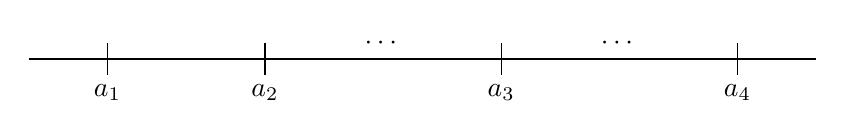
\begin{tikzpicture}
        % Draw the main line
        \draw[thick] (0,0) -- (10,0);
        
        % Draw and label the points
        \foreach \x/\label in {1/$a_1$, 3/$a_2$, 6/$a_3$, 9/$a_4$} {
            \draw (\x,0.2) -- (\x,-0.2); % Ticks
            \node[below] at (\x,-0.2) {\label}; % Labels
        };
        
        % Dots in between
        \node at (4.5,0.2) {$\cdots$};
        \node at (7.5,0.2) {$\cdots$};
    \end{tikzpicture}
    \caption{Possible ordering of the ancestors}
    \label{fig:order_of_ancestors}
\end{figure}

Now the question is, where can we place the elements of each unrelated tree. Before, $a_1$ we can only put nodes that are in the $u_5$ or $u_6$ subtree. Before $a_2$ we can put the same elements, plus $u_1$. In general, before a node $a_i$ we will be able to put all the nodes that are included in an $unrelated \ tree$ that it has root $ur$ such that $ur$ is a root or $a_j$ is the parent of $u_r$, with $j<i$. Now we want to turn this into a recursive formula so that we can use dynamic programming to solve this problem, as there are going to be multiple instances of overlapping problems. \\
For the algorithm, what we will be doing will in each step will be:
\begin{enumerate}
    \item Define where are we going to place the next ancestor. 
    \item Select how many nodes from each unrelated tree we are going to use to fill all the positions.
    \item Remove the selected nodes from our possible options to choose from. 
    \item Start the recursion again. 
\end{enumerate}
The parameters of the function will be:
\begin{itemize}
    \item $p$: position in which the last ancestor was placed
    \item $i$: index of the ancestor that we are going to place
    \item $nodesPerAncestor$: a list which has, in the $i-th$ position, the number of nodes to the left of the unrelated tree of $a_i$.
        \begin{itemize}
            \item Because of the slight improvement mentioned in \ref{slight_improvement} there will only be one tree under each $a_i$, since they are being merged into one. 
         \end{itemize}
\end{itemize}
We will also have some auxiliary functions: 
\begin{itemize}
    \item $\mathrm{possibleCombinations}(l,i,nodesPerAncestor) \ \text{or} \ pb$, which returns all the possible ways that you can sum the first $i$ elements of $nodesPerAncestor$ to obtain $l$. 
        \begin{itemize}
            \item For example, $\mathrm{possibleCombinations}(4,2,[10,2,6,7, \dots])= [[4,0], [3,1], [2,2]]$. 
        \end{itemize}
    \item $\mathrm{hasPlaced}(placedNodes, nodesPerAncestor) \ \text{or} \ hp$, returns a list $l$ which has in the $i-th$ position the element $l[i]= nodesPerAncestor[i] - placedNodes[i]$.
    \item $\mathrm{canPlace}(nodesPerAncestor, i) \ \text{or} \ cp$, returns the sum of the first $i$ elements of $nodesPerAncestor$.
\end{itemize}
Using this logic, our function will be like this: 

\label{formula:left_possible_orders}
%  \[
%     \leftPossibleOrders(p,i,npa) = 
%     \begin{cases} 
%     \sum_{comb \in pb(cp(i,npa),i, npa)} \binom{ sum(comb)}{comb_1, \ldots, comb_i} & \text{if $|A|=i$} \\
%     \sum_{s=p}^{p+cp(i,npa)} \sum_{comb \in pb(s-p-1,i, npa)} (\binom{ sum(comb)}{comb_1, \ldots, comb_i} * \leftPossibleOrders(s,i+1,hp(comb, npa))  & \text{otherwise}
%     \end{cases}
% \]

 \[
    \leftPossibleOrders(p,i,npa) = 
    \begin{cases} 
    \sum_{comb \in pb(cp(i,npa),i, npa)} \binom{ sum(comb)}{comb_1, \ldots, comb_i} & \text{if $|A|=i$} \\[2ex]
    \begin{aligned}
    &\sum_{s=p}^{p+cp(i,npa)} \sum_{comb \in pb(s-p-1,i, npa)} \Big(\binom{ sum(comb)}{comb_1, \ldots, comb_i} \\
    &  * \leftPossibleOrders(s,i+1,hp(comb, npa)\Big)
    \end{aligned}
    & \text{otherwise}
    \end{cases}
\]


%Esto en realidad es más complejo, hay algunas transformaciones que se tienen que hacer a left. ¿Las anoto o no tiene sentido? (Es lo que se hace en leftElementsOfClasses en el código)

In the otherwise case, the $s-p-1$ is the number of positions that we need to fill between the $a_i$ that we are placing and the $a_{i-1}$ that was placed before. Now with all this function defined, the call that will solve $leftOrders(A, left)$ will be $f(0,0,left)$. We implemented this function using dynamic programming, so we won't be solving the overlapping problems twice. 


\subsection{Time complexity}
%TODO: ¿Esta es la idea? ¿Cuánto más formal debería ser? ¿Cuánto mejor lo debería escribir? ¿Busco una cota un poco más fina?
Let $n$ be the number of nodes of the causal digraph $G$, $r$ the root of $G$ and $eq$ the number of equivalence classes in $G$ for feature $x_i$.

\subsubsection{Time complexity of \unrEqCl}

For calculating the complexity of \unrEqCl, defined in \ref{formula:unrelated_equiv_classes}, we are going to calculate how much each node costs and how many calls there are. $leftUnion$ and $rightUnion$ does 4 times $|n|$ operations of cost $O(1)$, 2 $\prod \ and \ \sum$. The multinomial coefficient is $O(n)$ in the worst case, so $leftUnion$ and $rightUnion$ will have a $O(n)$ time complexity. Then we need to bound the number of $mix$ that will be created in each call, but because we are generating the equivalence classes here we know it will be bounded by $\#equivalenceClasses$. We will also call this function at most $n$ times, once for each node. That leaves us with a total time complexity of $O(n^2 * \#equivalenceClasses)$.

\subsubsection{Time complexity of \#eqClass}

First, we need to calculate the time complexity of $rightSize$, which is $O(n)$. We have the multinomial coefficient, which takes $O(n)$ time, the $\prod$ which is $O(n)$ cause $|UR|<n$ and $\#topo(x_i)$ which can be implemented in $O(n)$. Then the sum of 3 operations that take $O(n)$ time is $O(n)$. 

%TODO: Revisar la cota de complejidad para \#topo(x_i), cómo mucho va a ser  $O(n^2) igual$

We also have to calculate the complexity of \leftPossibleOrders, defined in \ref{formula:left_possible_orders}, for that we need to know how much does it cost to calculate each node and how many possible states there are.

Let's start with the possible states. We have the parameters $i$, $p$ and $nodesPerAncestor$. $i$ has $|A|$ possible values, which in the worst case is $O(n)$. $p$ can take $O(n)$ possible values in the worst case, because a topological order can have at most $n$ nodes. Now we have to  calculate the number of possible states for $nodesPerAncestor$: 

For each $i$ position, we are going to have the number of nodes to the left of the unrelated trees under $a_i$. Let $size(ut_i)$ be the size of the unrelated tree $ut_i$ under node $a_i$ (if there is none, it is 0). For the $i-th$ position, we have $size(ut_i)$ possible values. But with formula \ref{formula:number_of_equiv_classes} we know that $\numEqCl(ut_i) > size(ut_i)$, that means that the possible values of $nodesPerAncestor$ are bounded by $\prod_{i=0}^{|A|} size(ut_i) < \prod_{i=0}^{|A|} numEqCl(ut_i)$. And knowing how we calculate all the equivalence classes sizes in \ref{formula:number_of_equiv_classes} we know that $\prod_{i=0}^{|A|} numEqCl(ut_i) < numEqCl(r) = \text{number of equivalence classes}$. With that, we can conclude that $\# possible \ values \ of \ npa < number \ of \ equivalence \ classes$. 

%TODO: Creo que cometí un crimen de lesa humanidad metiendo la notación O acá, pero después lo corrijo.
Then we have that the number of states is in the order of $values(i) * values(p) * values(npa) = O(n) * O(n) * \#equivalenceClasses = O(n^2 * \#equivalenceClasses)$.

Now we need to calculate how much does each node costs. The multinomial coefficient is $O(n)$, because the maximum size $comb$ can take is $n$ and multiplying is $O(1)$. So the number of sums will determine our complexity. $s$ can take at most $\sum_j^i size(ut_j)$ values in each iteration, and that's bounded by $n$. The question is how many values can $\mathrm{possibleCombinations}(l,i,nodesPerAncestor)$ can take. We know that for each result $res$ such that $res \in pb(l,i,npa), \forall 0<j<|res|, 0<res[j]<npa[j]$. So using a similar argument as the one in $nodesPerAncestor$ we can conclude that $pb(l,i,npa) < \#equivalenceClasses$. Concluding that the cost of calculating each state is $O(n^2 * \#equivalenceClasses)$.
Now we need to calculate how much does each node costs. The multinomial coefficient is $O(n)$, because the maximum size $comb$ can take is $n$ and multiplying is $O(1)$. So the number of sums will determine our complexity. $s$ can take at most $\sum_j^i size(ut_j)$ values in each iteration, and that's bounded by $n$. The question is how many values can $\mathrm{possibleCombinations}(l,i,nodesPerAncestor)$ can take. We know that for each result $res$ such that $res \in pb(l,i,npa), \forall 0<j<|res|, 0<res[j]<npa[j]$. So using a similar argument as the one in $nodesPerAncestor$ we can conclude that $pb(l,i,npa) < \#equivalenceClasses$. Concluding that the cost of calculating each state is $O(n^2 * \#equivalenceClasses)$.

That leaves us with a time complexity of $O(n^4 * \#equivalenceClasses^2)$ for \leftPossibleOrders and $\#eqClass$

\subsubsection{Final time complexity}

The complexity of our algorithm will be $O(\unrEqCl) + \#equivalenceClasses * O(\#eqClass)$. Since first, we need to run  $\unrEqCl$ to obtain the equivalence classes we are going to merge. And then for each equivalence class that will be created, we need to calculate it's size and it's elements. Then the complexity will be $O(n^2 * \#equivalenceClasses)$ + $O(n^4 * \#equivalenceClasses^3)$ = $O(n^4 * \#equivalenceClasses^3)$. 

\subsection{Approximate aproach}

\subsection{Experimentation}

%TODO: Compare the naive way of doing it (computing all of the topological sorts) vs equivalence classes for the CHILD bayesian network






\section{ASV with equivalence classes}


\section{Tareas}

Falta escribir:

\begin{itemize}
    \item Sección 2.3.2 (Mean prediction in decomposable)
    \item Sección 2.3.3 (Approximate mean prediction).
\end{itemize}

\bibliographystyle{plain}
\bibliography{biblio}




\end{document}
